
We implemented our method
and compared it with the traditional methods.
\\
We use leave-one-out cross-validation (LOOCV) method (using a single data from the original dataset as the test data, and the remaining data as the training data. This is repeated such that each data in the dataset is used once as the test data) to find error rate of each methods.\\
\begin{flushleft}
\textbf{Traditional Distance Function Result:}\\
\end{flushleft}

\begin{enumerate}

\item Euclidean Distance : It produces Error Rate = 0.64273 
\item Cosine Similarity : It produces Error Rate = 0.54636
\item Dynamic Time Warping: 
Error Rate = 0.63\\
We improve the performance(computation time) of DTW by using UCR Suite (code provide in cpp by Eamonn in their website). We modify their code to integrate them in our system. We experimented by setting size of warping windows to be +/-5\%. When we stripping the 0 from begin and end of time series, the result got slightly better (Error Rate = 0.60) but still the result is not as good as we originally expected (probably because DTW try to match bursty noise) so we decide to focus on signal transformation for now.
\item Cepstrum: It produces Error Rate = 0.43636 
\end{enumerate}

\begin{flushleft}
\textbf{Custom Distance Function Result:}\\
\end{flushleft}

\begin{enumerate}
\item Shift time series to match the position of sound occurrence
The below figure is a time series for insect sound in class 9
\begin{figure}[H]
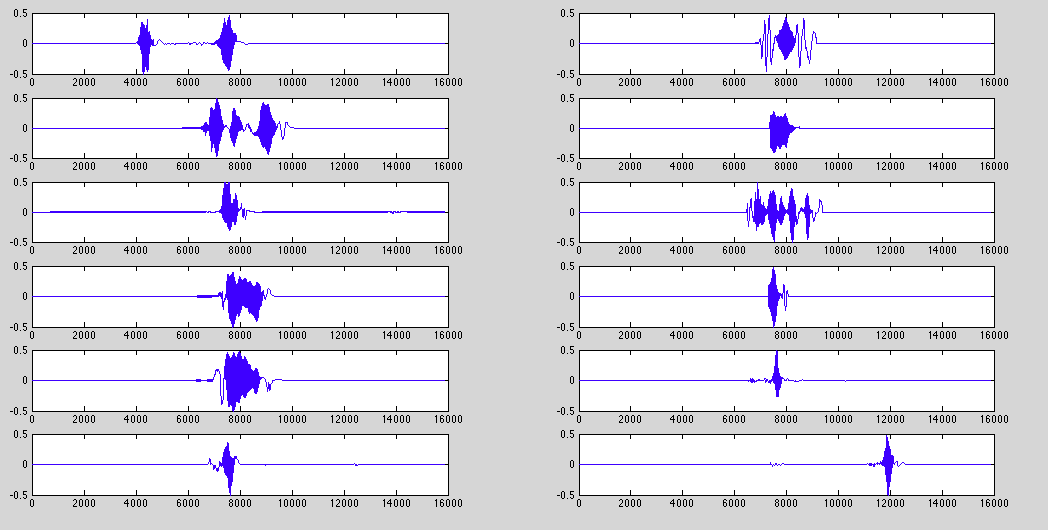
\includegraphics[scale=.4]{PIC/class9raw.png}
\caption{Raw data for class 9}
\end{figure}
We can clearly see that the wave in the first and the last time series are in differrent position than others. Thus these two are highly likely to be misclassified. We develop algorithm to shift the time series to begin at appoximately same location to make our distance function be more accurate.
The algorithm we designed is as follow:
\begin{enumerate}
\item find the first local maxima point that has height greater than 1/3 of global maxima
\item shift the time series to the left matching position of the discovered local maxima to position 1500.
\item keep only 4500 first time ticks because no time series has non zero elements span more than 4000 time tics.\\
Below is the times series in figure 1 after apply this algorithm
\end{enumerate}
\begin{figure}[H]
\centering
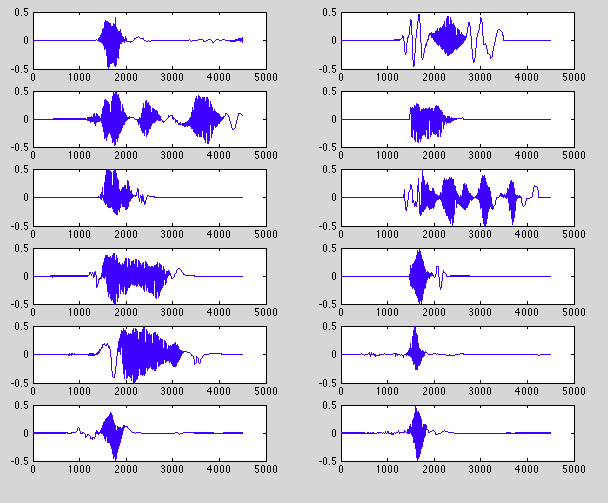
\includegraphics[scale=.4]{PIC/class9shift.png}
\caption{time seires for class 9 insect after shifting}
\end{figure}
The new time series above have approximately same starting position and we can also reduce the dimension by 2/3 too. Using Euclidean distance and Cosine distance on the preprocessed time series, we get this result
Euclidean Distance error rate: 0.56727
Cosine Distance error rate: 0.52909 

The result improves from 0.64 to 0.56 for ED and 0.54 to 0.52 for cosine)


\item Preprocessing audio signal by doing Discreet Fourier Transform.\\

We use Fast Fourier Transform on input signal. Then we compare the distance between transformed signal using Euclidean distance and Cosine similarity distance. The result are as follows: 

\begin{enumerate}
\item Euclidean Distance : It produces Error Rate = 0.40636
\item Cosine Similarity : It produces Error Rate = 0.40091
\end{enumerate}

The reason why the accurary of our classifier improves after doing Fourier Transform is because we can observe more significant trends in frequency domain rather than in time domain. For example, considering the raw time series plot of insect in class 1 below
\begin{figure}[H]
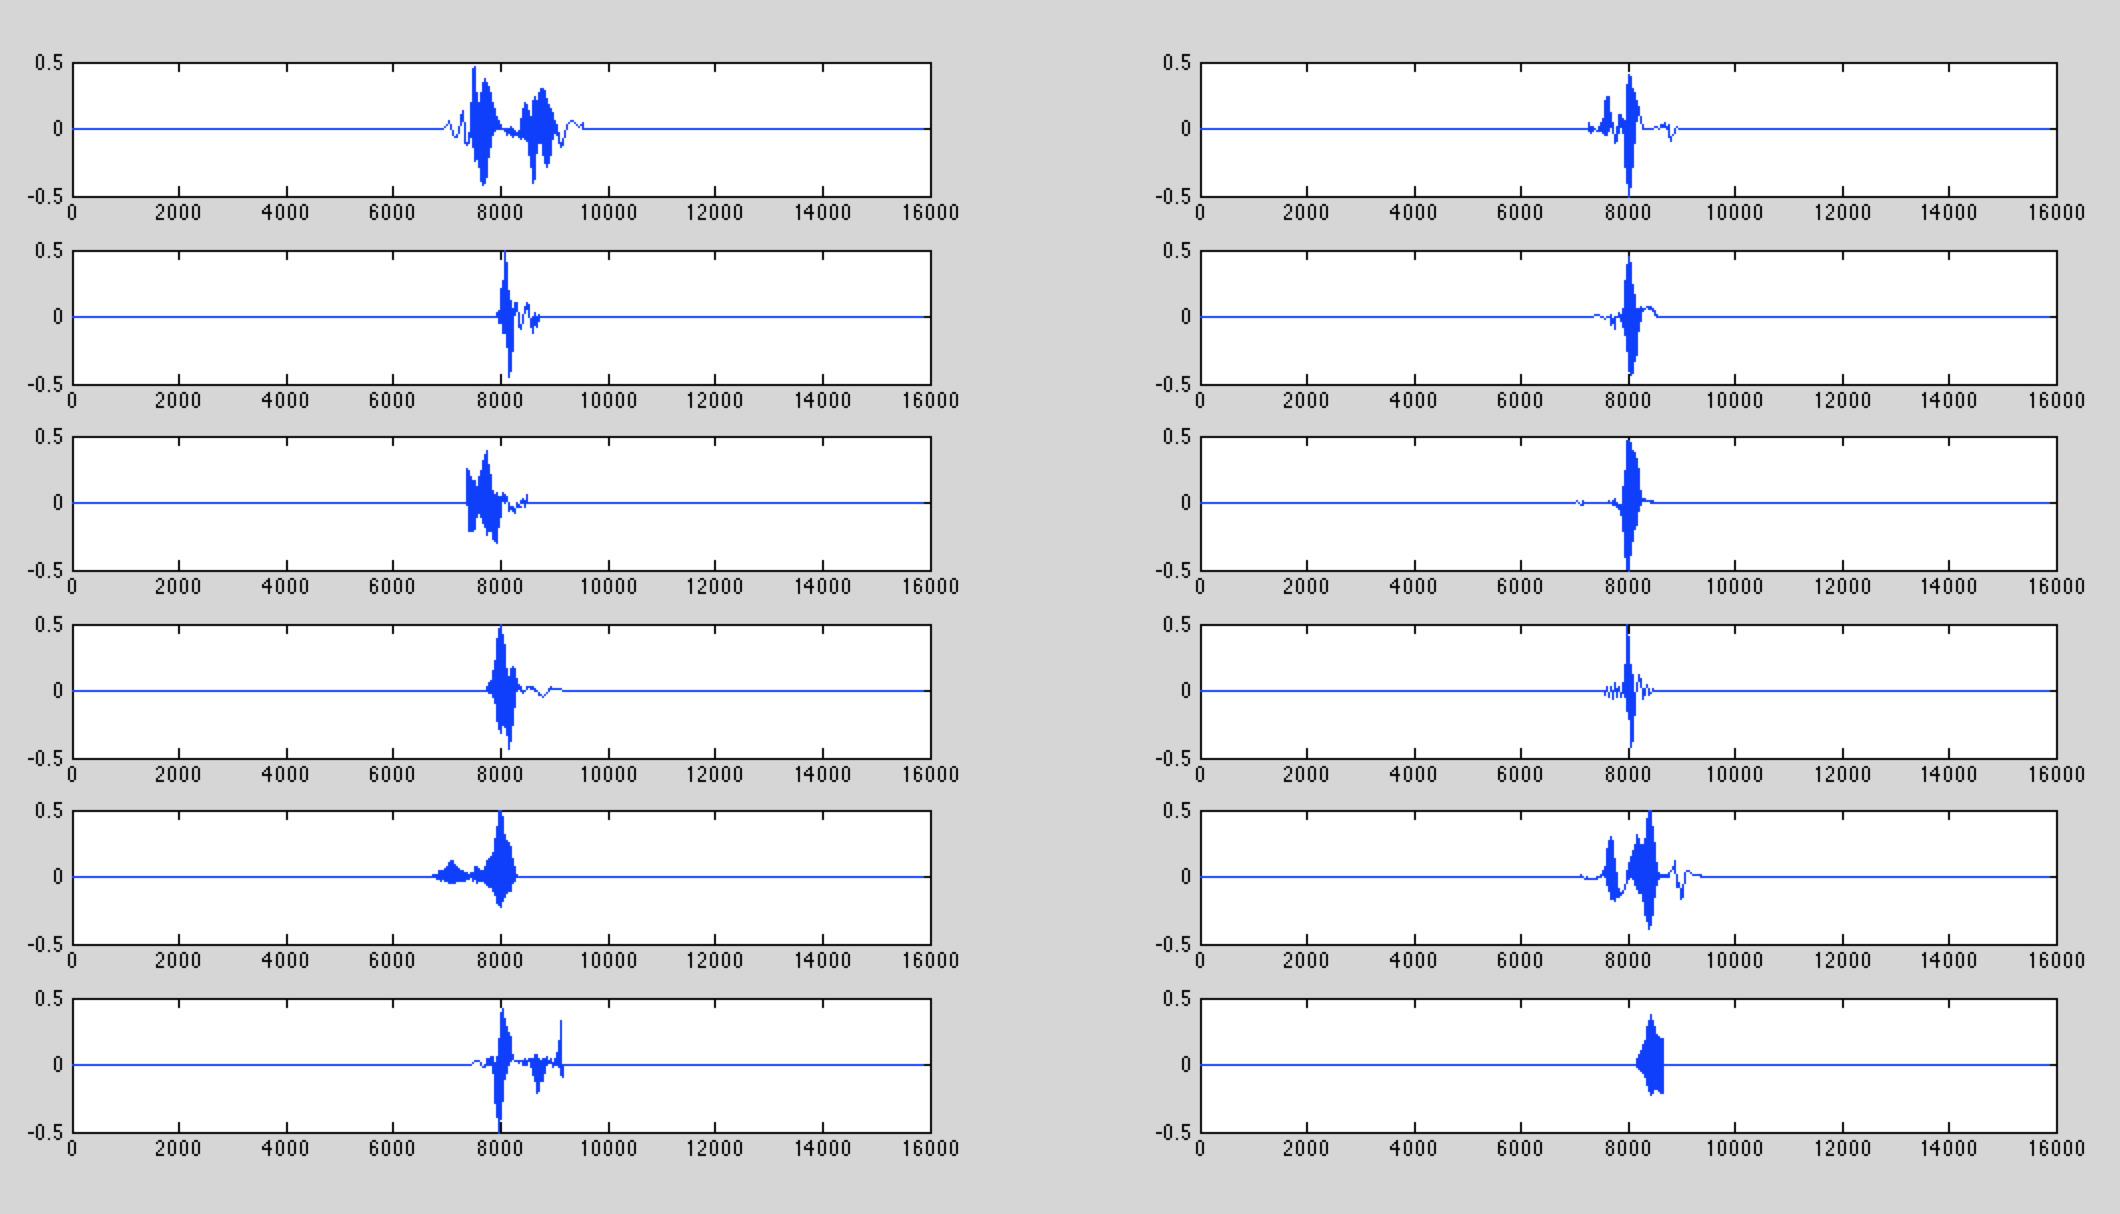
\includegraphics[scale=.4]{PIC/raw_class1.png}
\caption{Raw data for class 1}
\end{figure}
We can not really tell what is the common pattern between these time series. But if we consider the plot in frequency domain below:
\begin{figure}[H]
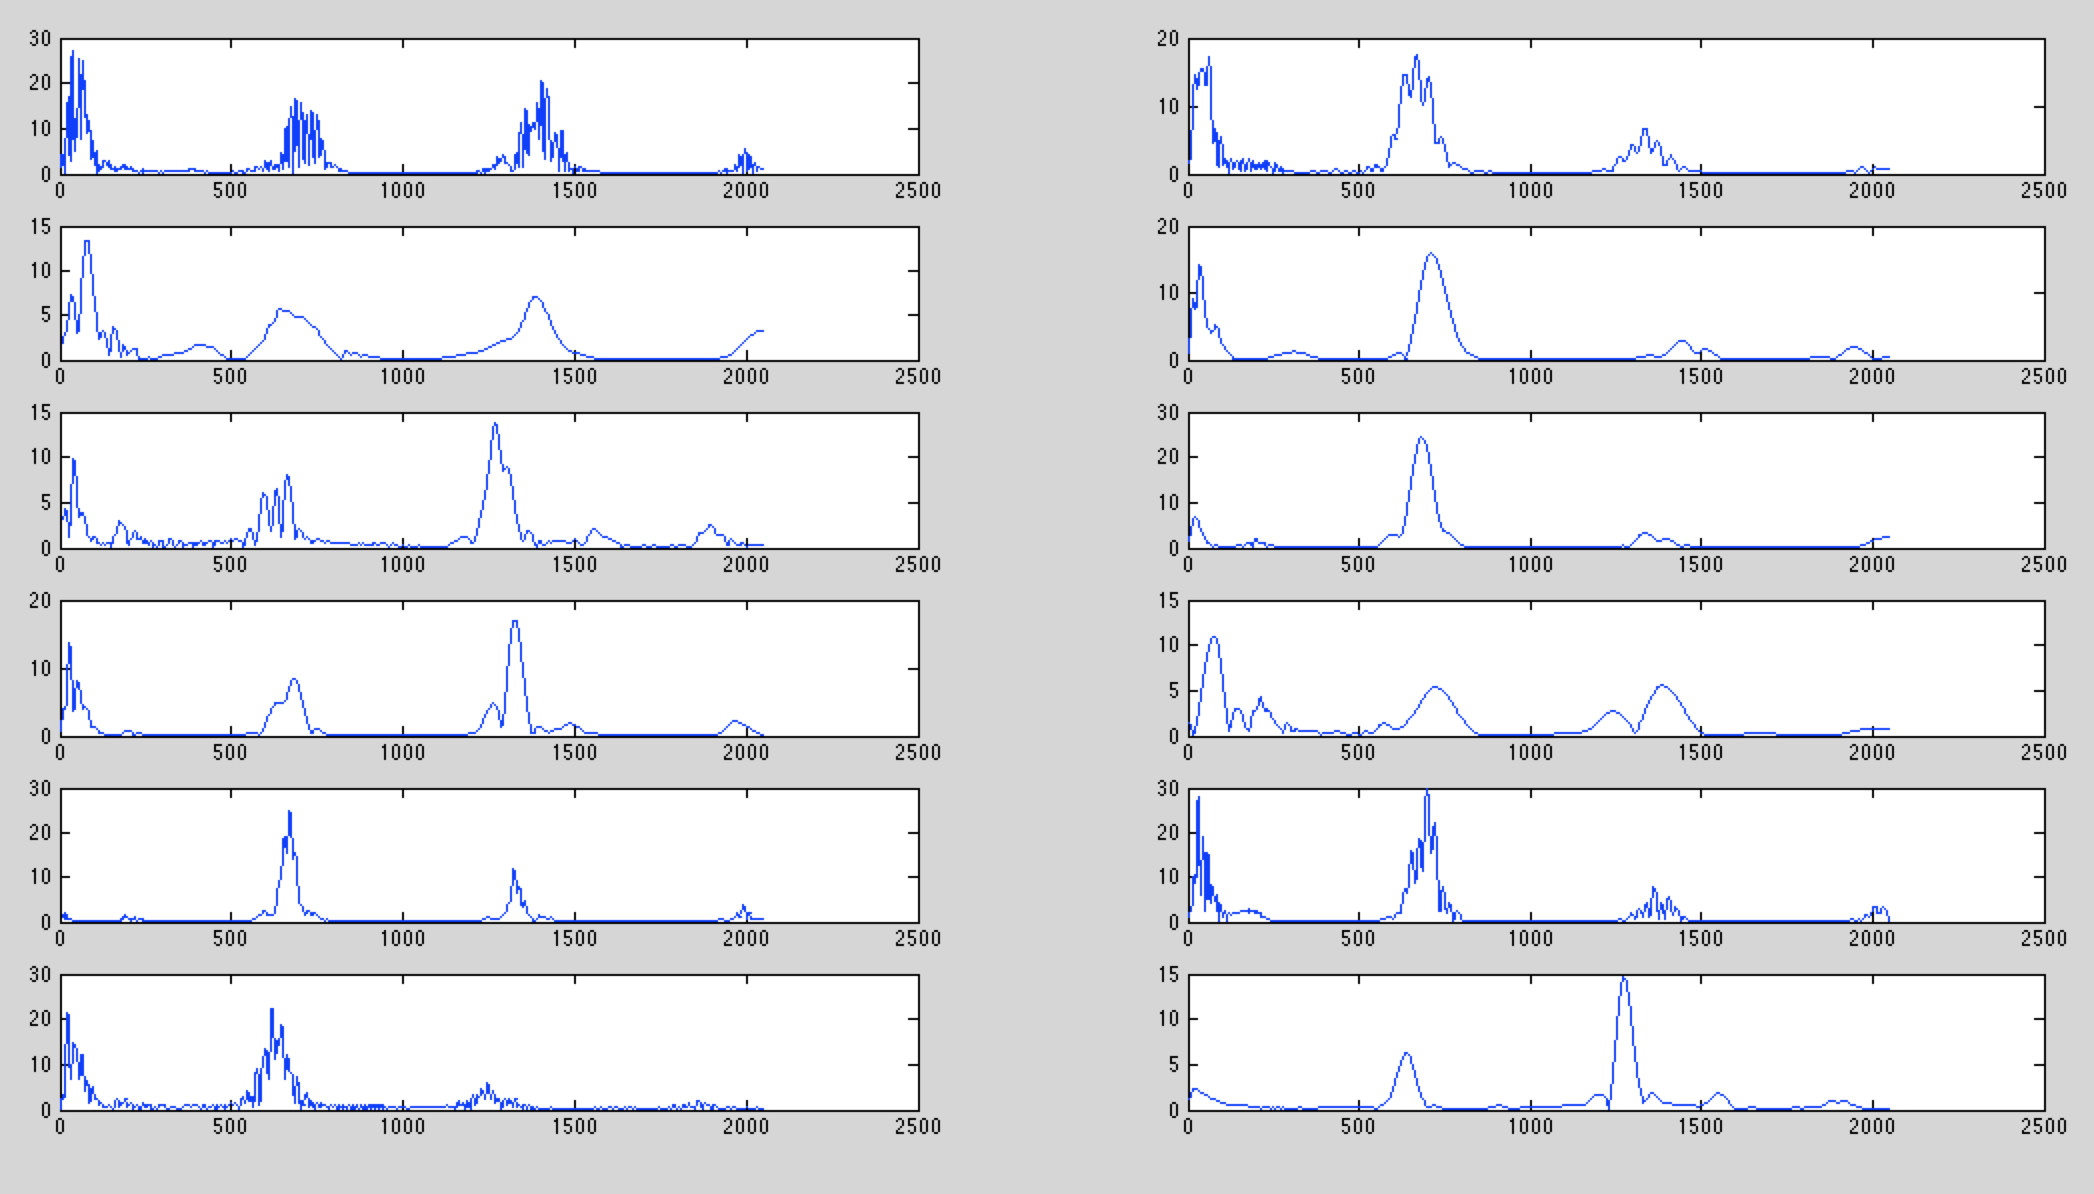
\includegraphics[scale=.4]{PIC/extracted_ffted_class1.png}
\caption{class 1 after fast fourier transform}
\end{figure}
We can observe that the position of major frequencies(first 2 or 3 peaks) is more or less similar in this class. Also Fourier Transform which doesn't capture the change in time is actually a favourable option in case that the start and end of each sounds is not in the same place. Thus apply simple distance function in frequency domain give us better result than in time domain. 

Moreover we tried using SVD to extract 20 strongest concepts from our transformed signal. Then used those 20 coefficient to compare the distance using cosine similarity. We got the error rate of 0.40182

\item Preprocessing audio signal by doing Multi-Level Wavelet Decomposition.\\

We tried using Daubechies-4 and Daubechies-12 wavelet decomposition at level in range 3 to 5. Then use all coefficients in every levels as features. We got the error rate at 0.54 +- 10\%. This means some coefficient do not have high saperatable ability (not good for classification use). Thus our plan for next step is to find a good way to do feature extractions. 

\item Preprocessing audio signal by doing Haar Wavelet Transformation, then extract feature, after that, apply Fast Fourier Transform algorithm on each time series.\\
The raw timeseries of class 1 is as below: (only show 12 of them)\\

\begin{figure}[H]

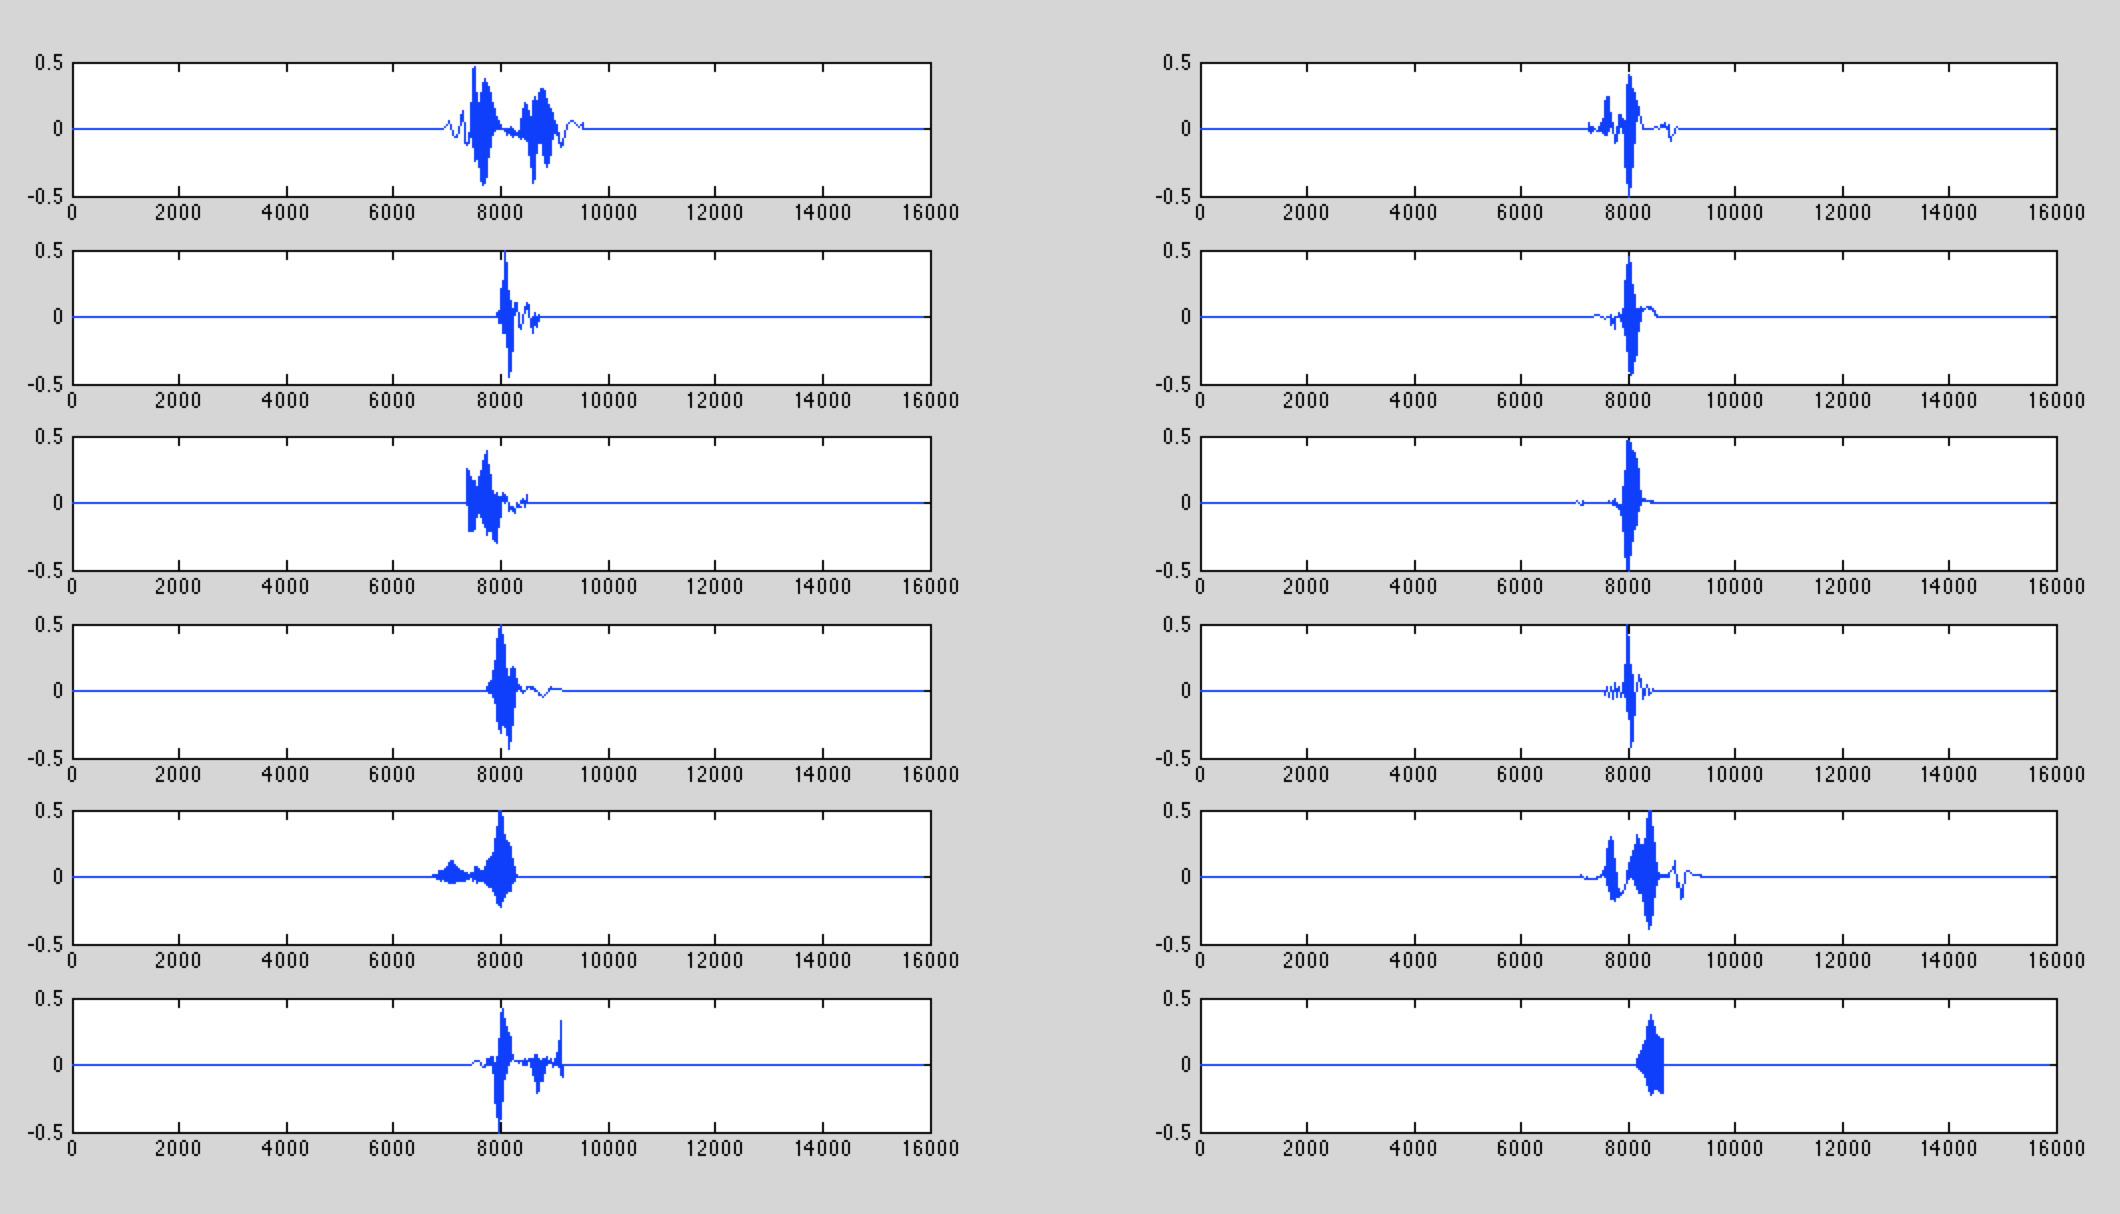
\includegraphics[scale=.4]{PIC/raw_class1.png}
\caption{Raw data for class 1}
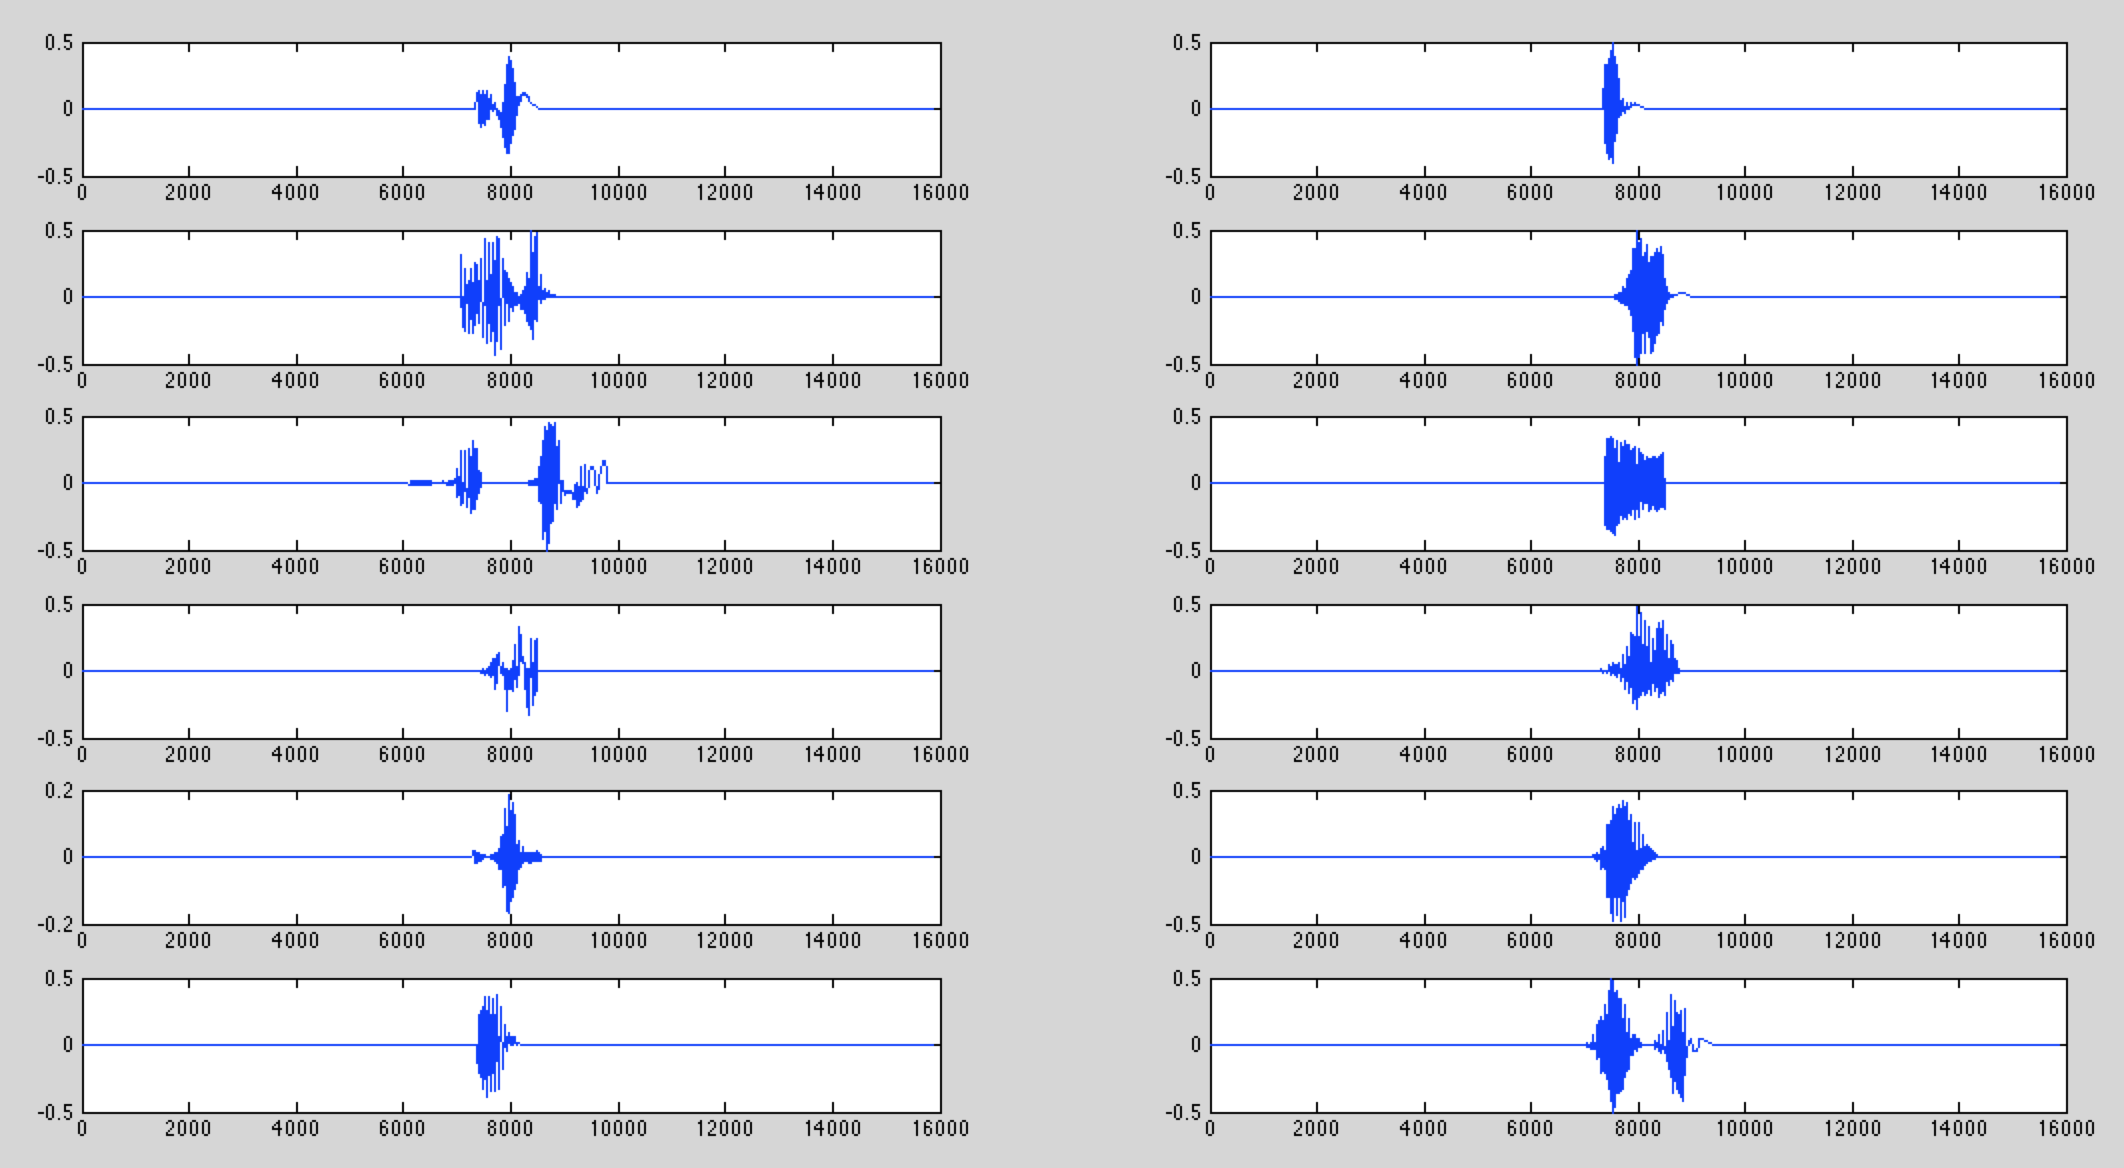
\includegraphics[scale=.4]{PIC/raw_class2.png}
\caption{Raw data for class 2}
\end{figure}


Through observation of the above two raw time series, we can not see any pattern within one class and can not tell apart two classes of time series.\\
Then we apply Haar wavelet transformation and extract features from timeseries.\\\\
For Wavelet Feature Extraction, 

We choose to use unsupervised classification to extract some feature.
For a time series, the features corresponding to higher scale keep more wavelet coefficients and have higher dimensionality compared to lower scale.
For a time series dataset having m time series,
when decreasing the scale from the highest scale to scale 0, discarding the wavelet coefficients within a scale with lower energy ratio will not decrease the sum of energy of all removed wavelet coefficients to a large scale. If a scale j satisfies 
$$\sum_{j=1}^{m}X_j^{2} < \sum_{j=1}^{m}X_{j-1}^{2}$$, removing the wavelet coefficients within this scale and higher scales achieves a local tradeoff of lower D and lower dimensionality for the dataset. If $$\sum_{j=1}^{m}X_j^{2}$$ within a scale is small, there will be lots of noise embedded within this scale, cutting off the wavelet coefficients within this scale can remove more noise. The algorithm[9] is described below:\\\\

\begin{figure}[H]

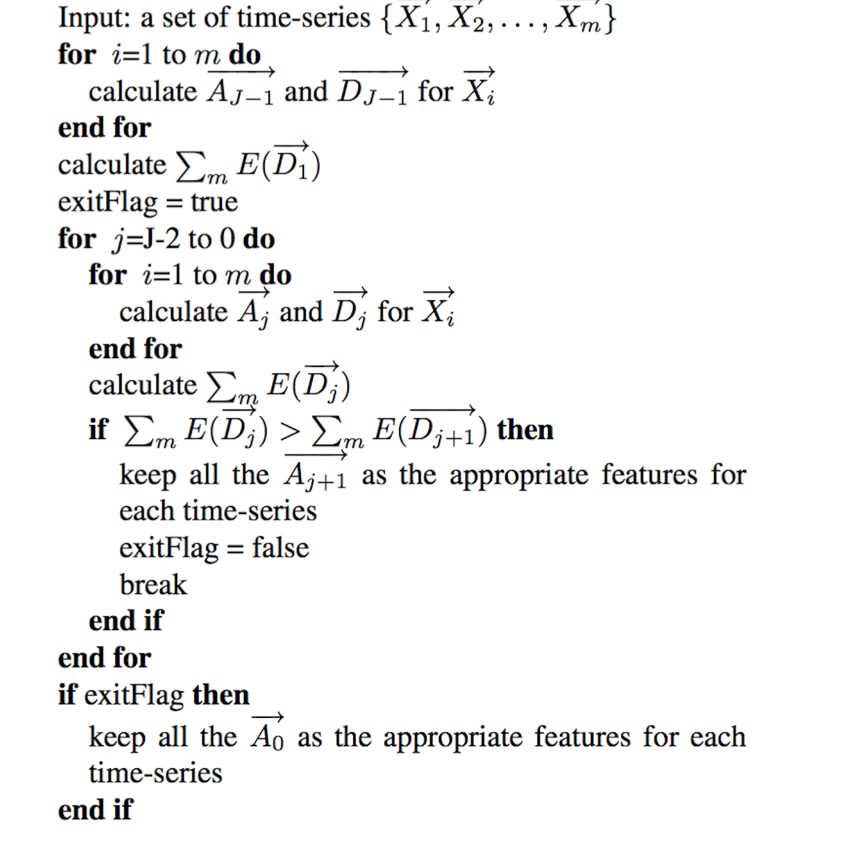
\includegraphics[scale=.7]{PIC/alg_feature_extraction.png}
\end{figure}

The processed timeseries are shown below:\\
\begin{figure}[H]
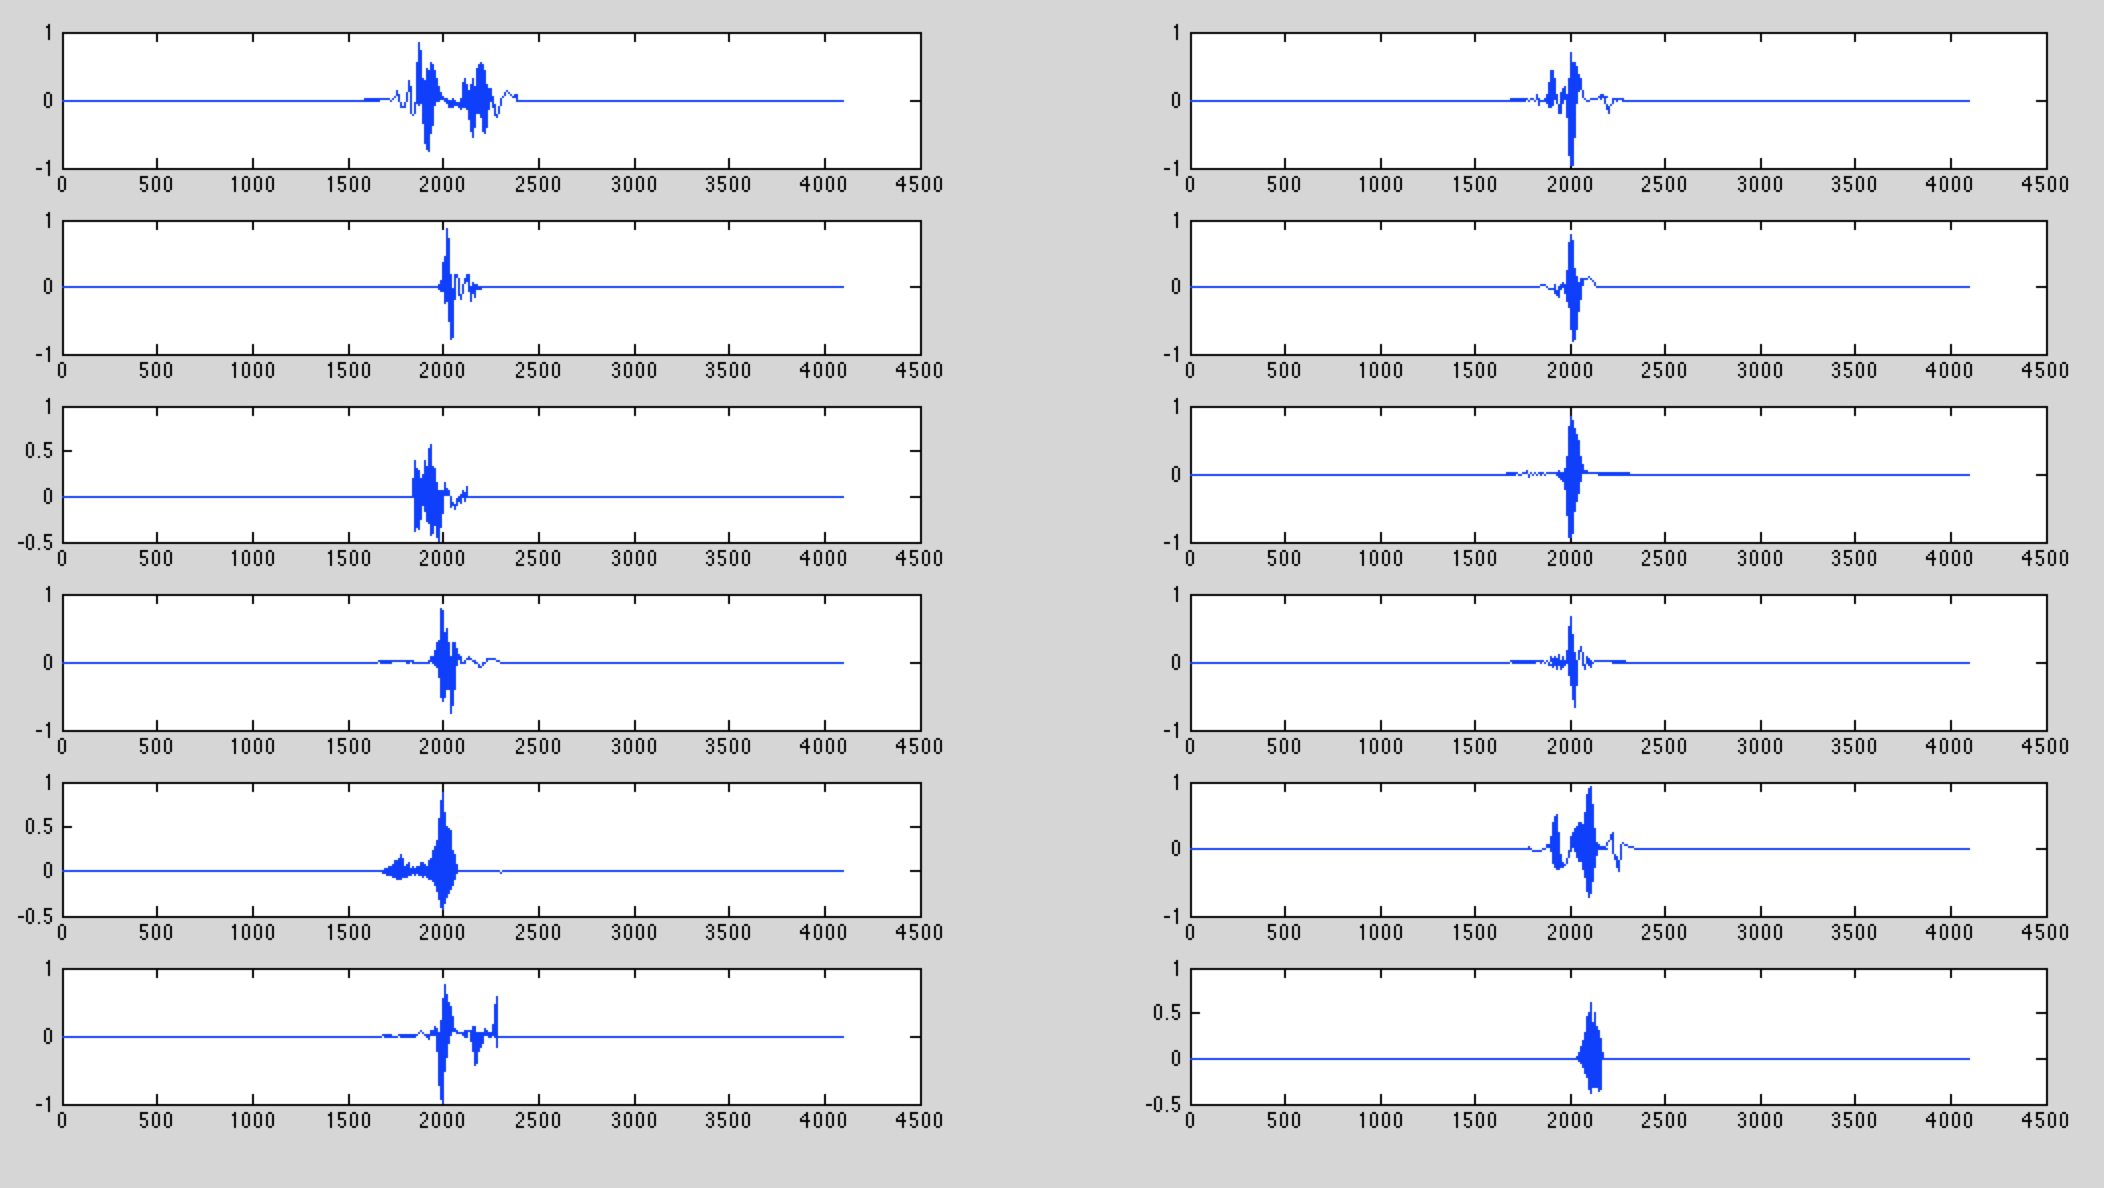
\includegraphics[scale=.4]{PIC/extracted_class1.png}
\caption{class 1 after wavelet transformation and feature extraction}

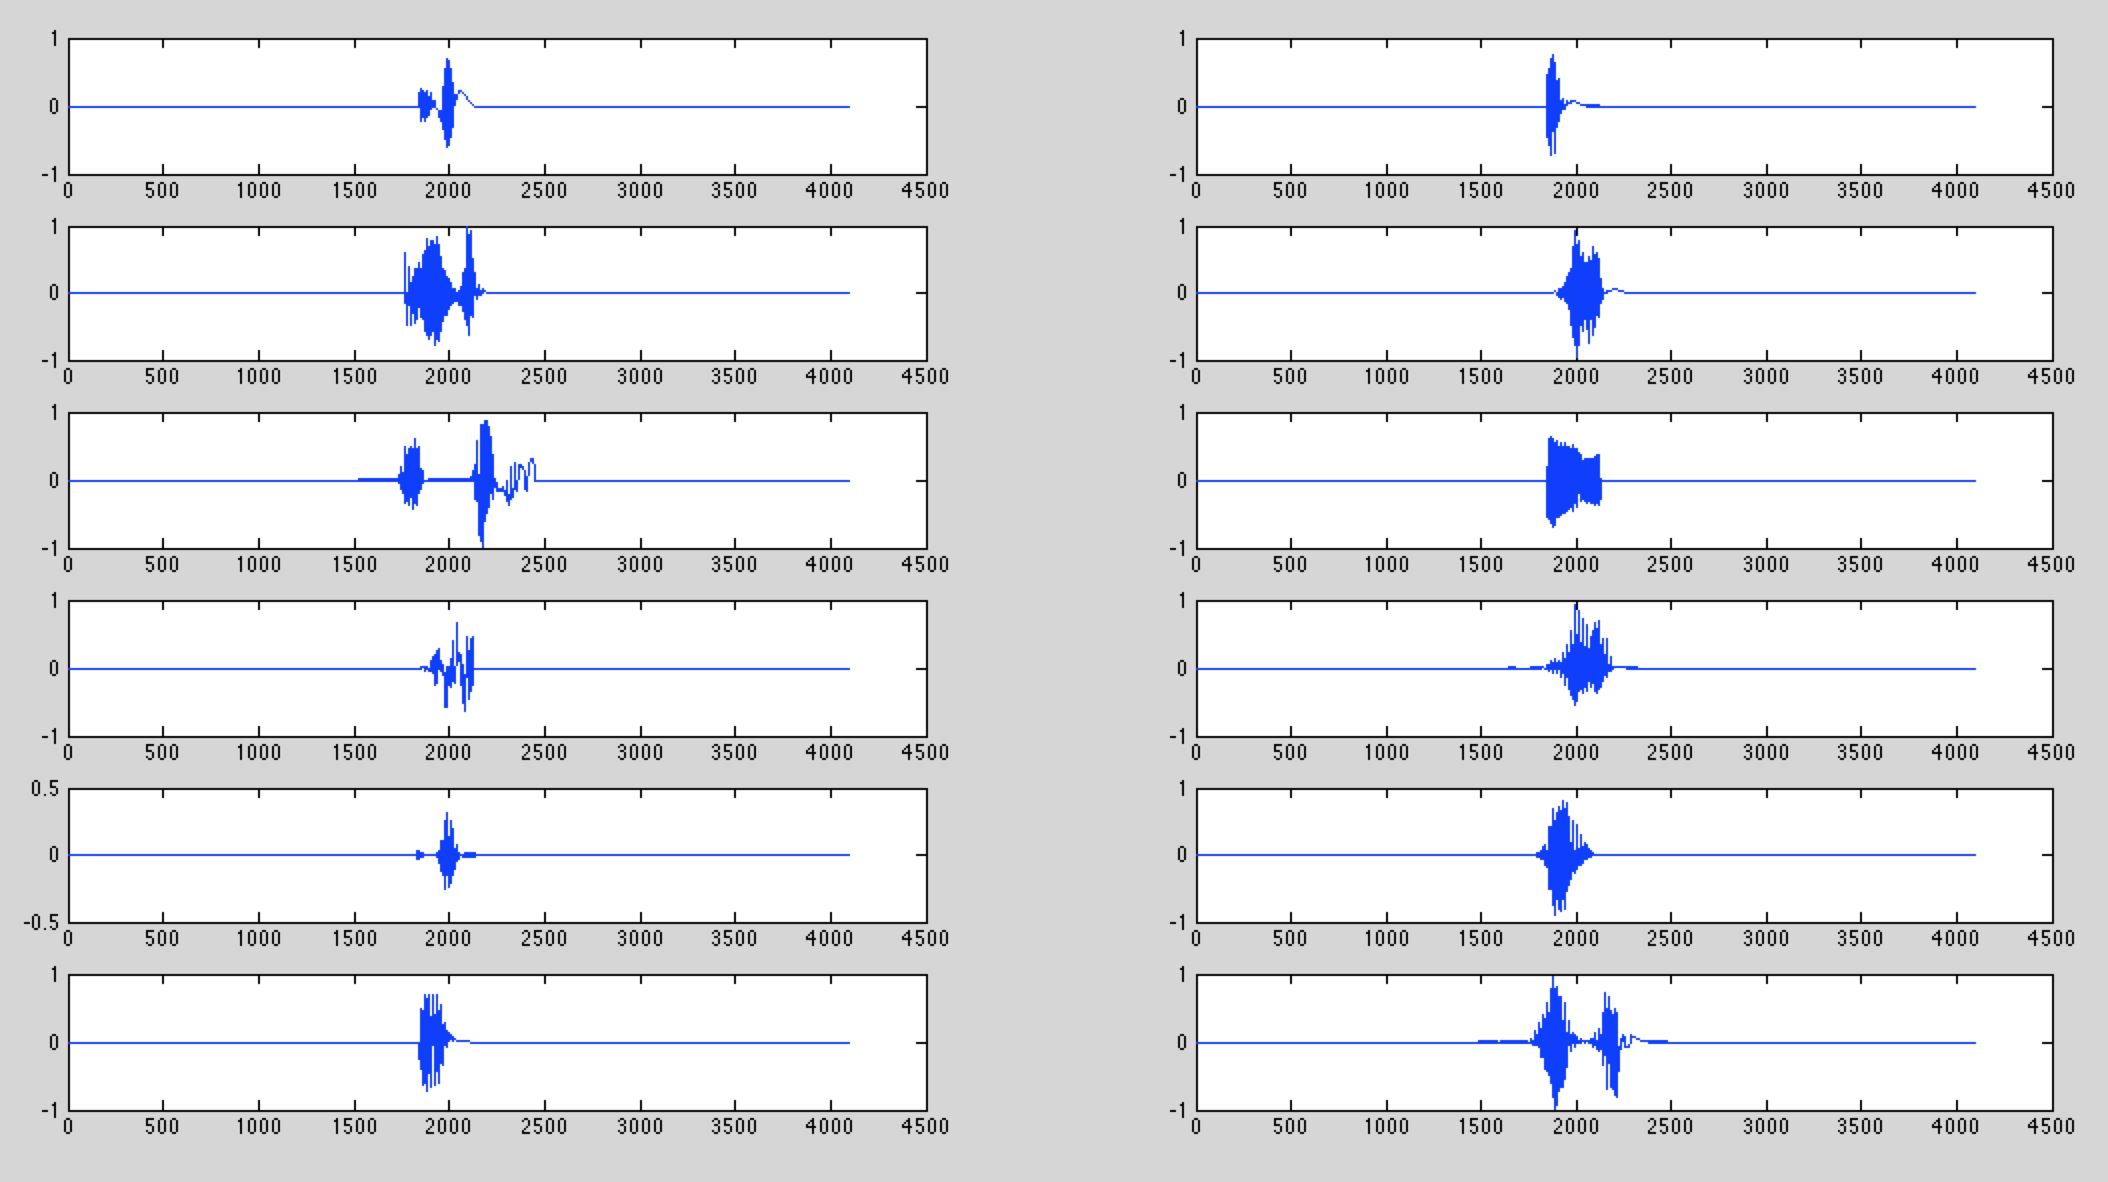
\includegraphics[scale=.4]{PIC/extracted_class2.png}
\caption{class 2 after wavelet transformation and feature extraction}
\end{figure}
We can observe that after the above steps, the dimension of timeserie is reduced and we kept the approximation as the feature of timeserie.\\
Now we need to find the frequency of wave from each timeseries, after apply Fast Fourier Transform Algorithm on the timeseries, we get the plots below(because FFT mirrors the plots, we choose to observe only half of each plot):\\
\begin{figure}[H]

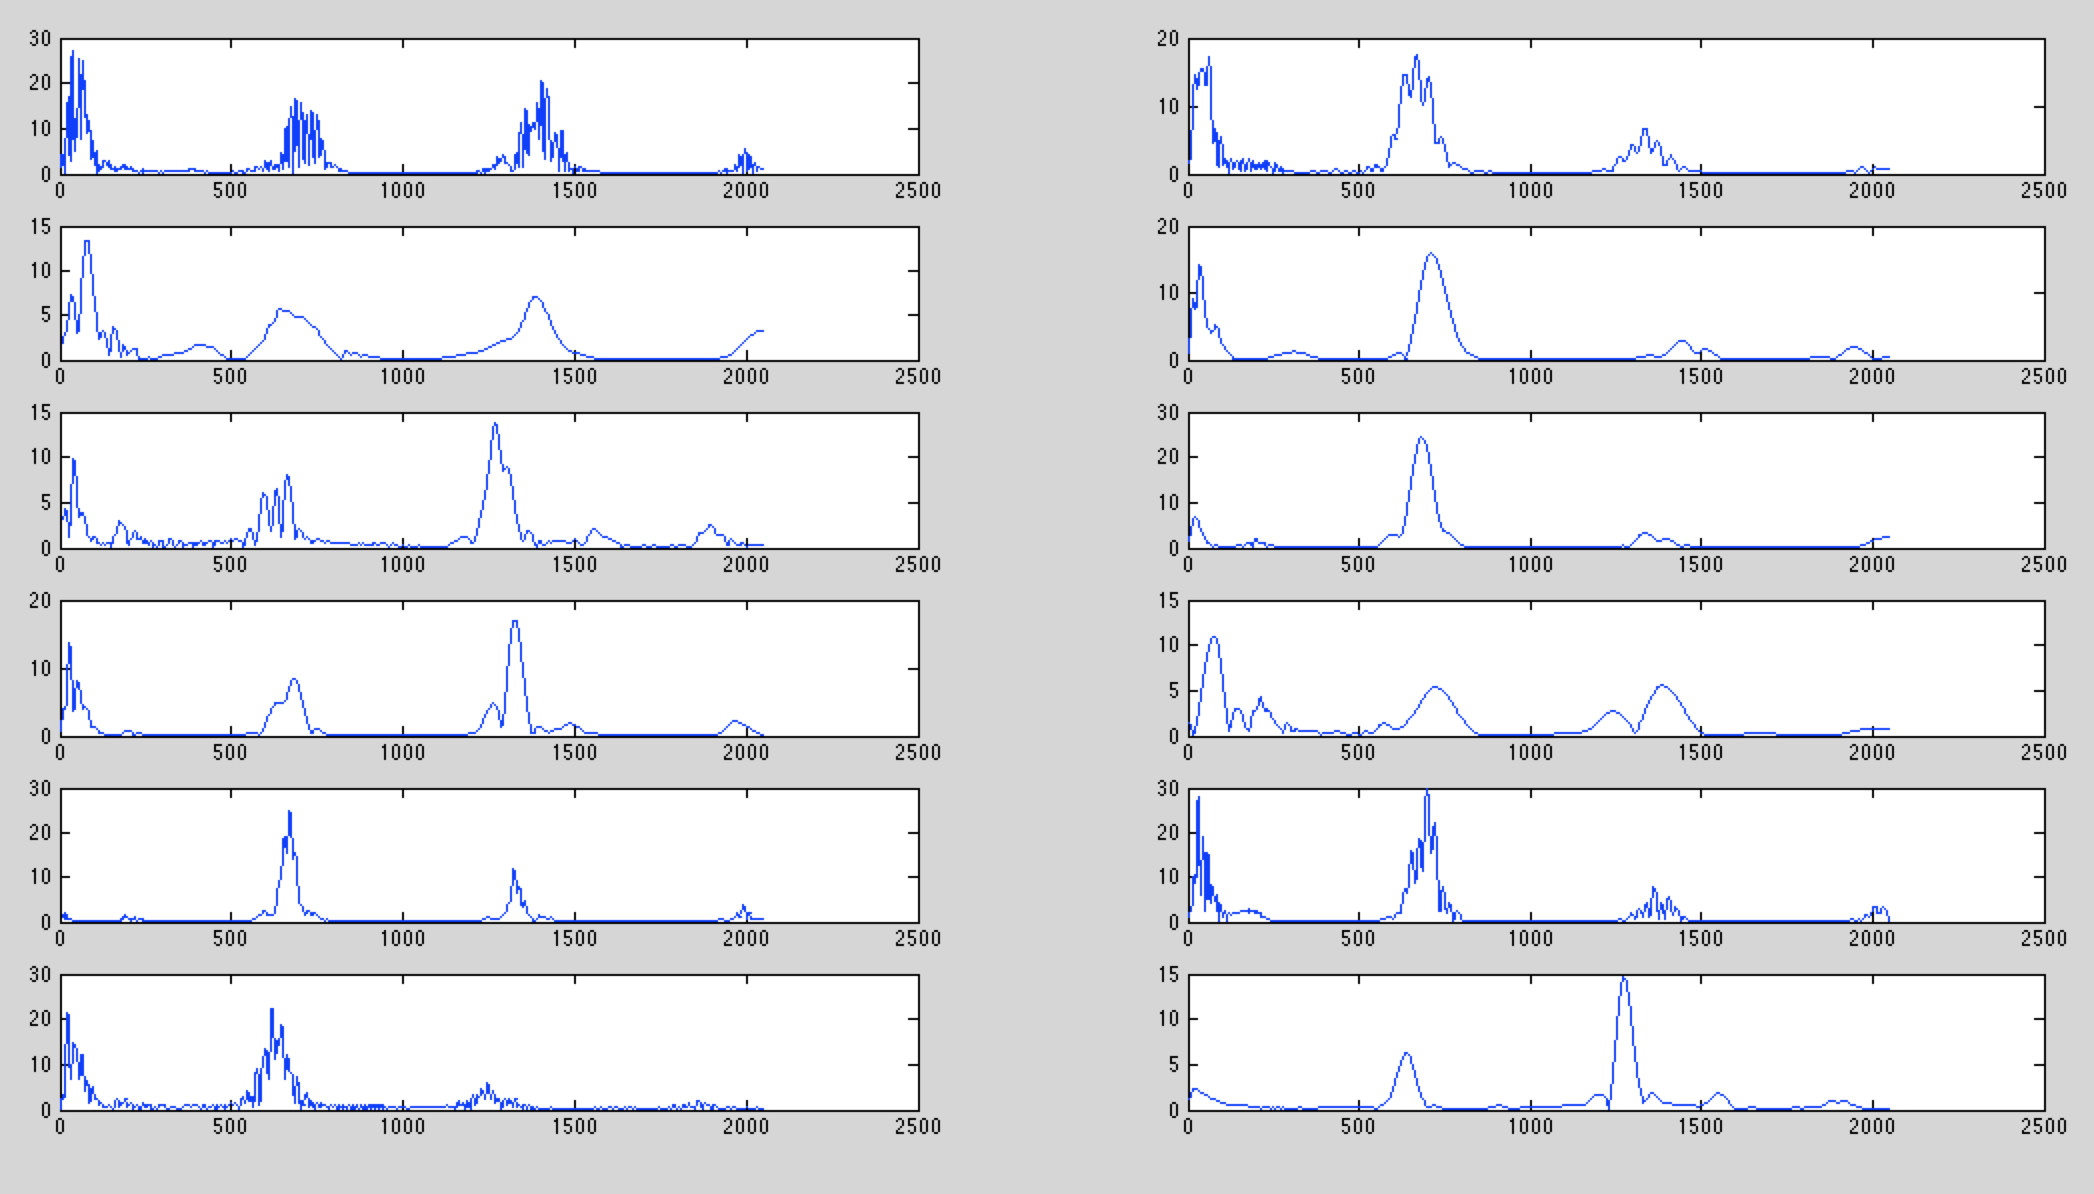
\includegraphics[scale=.4]{PIC/extracted_ffted_class1.png}
\caption{class 1 after fast fourier transform}

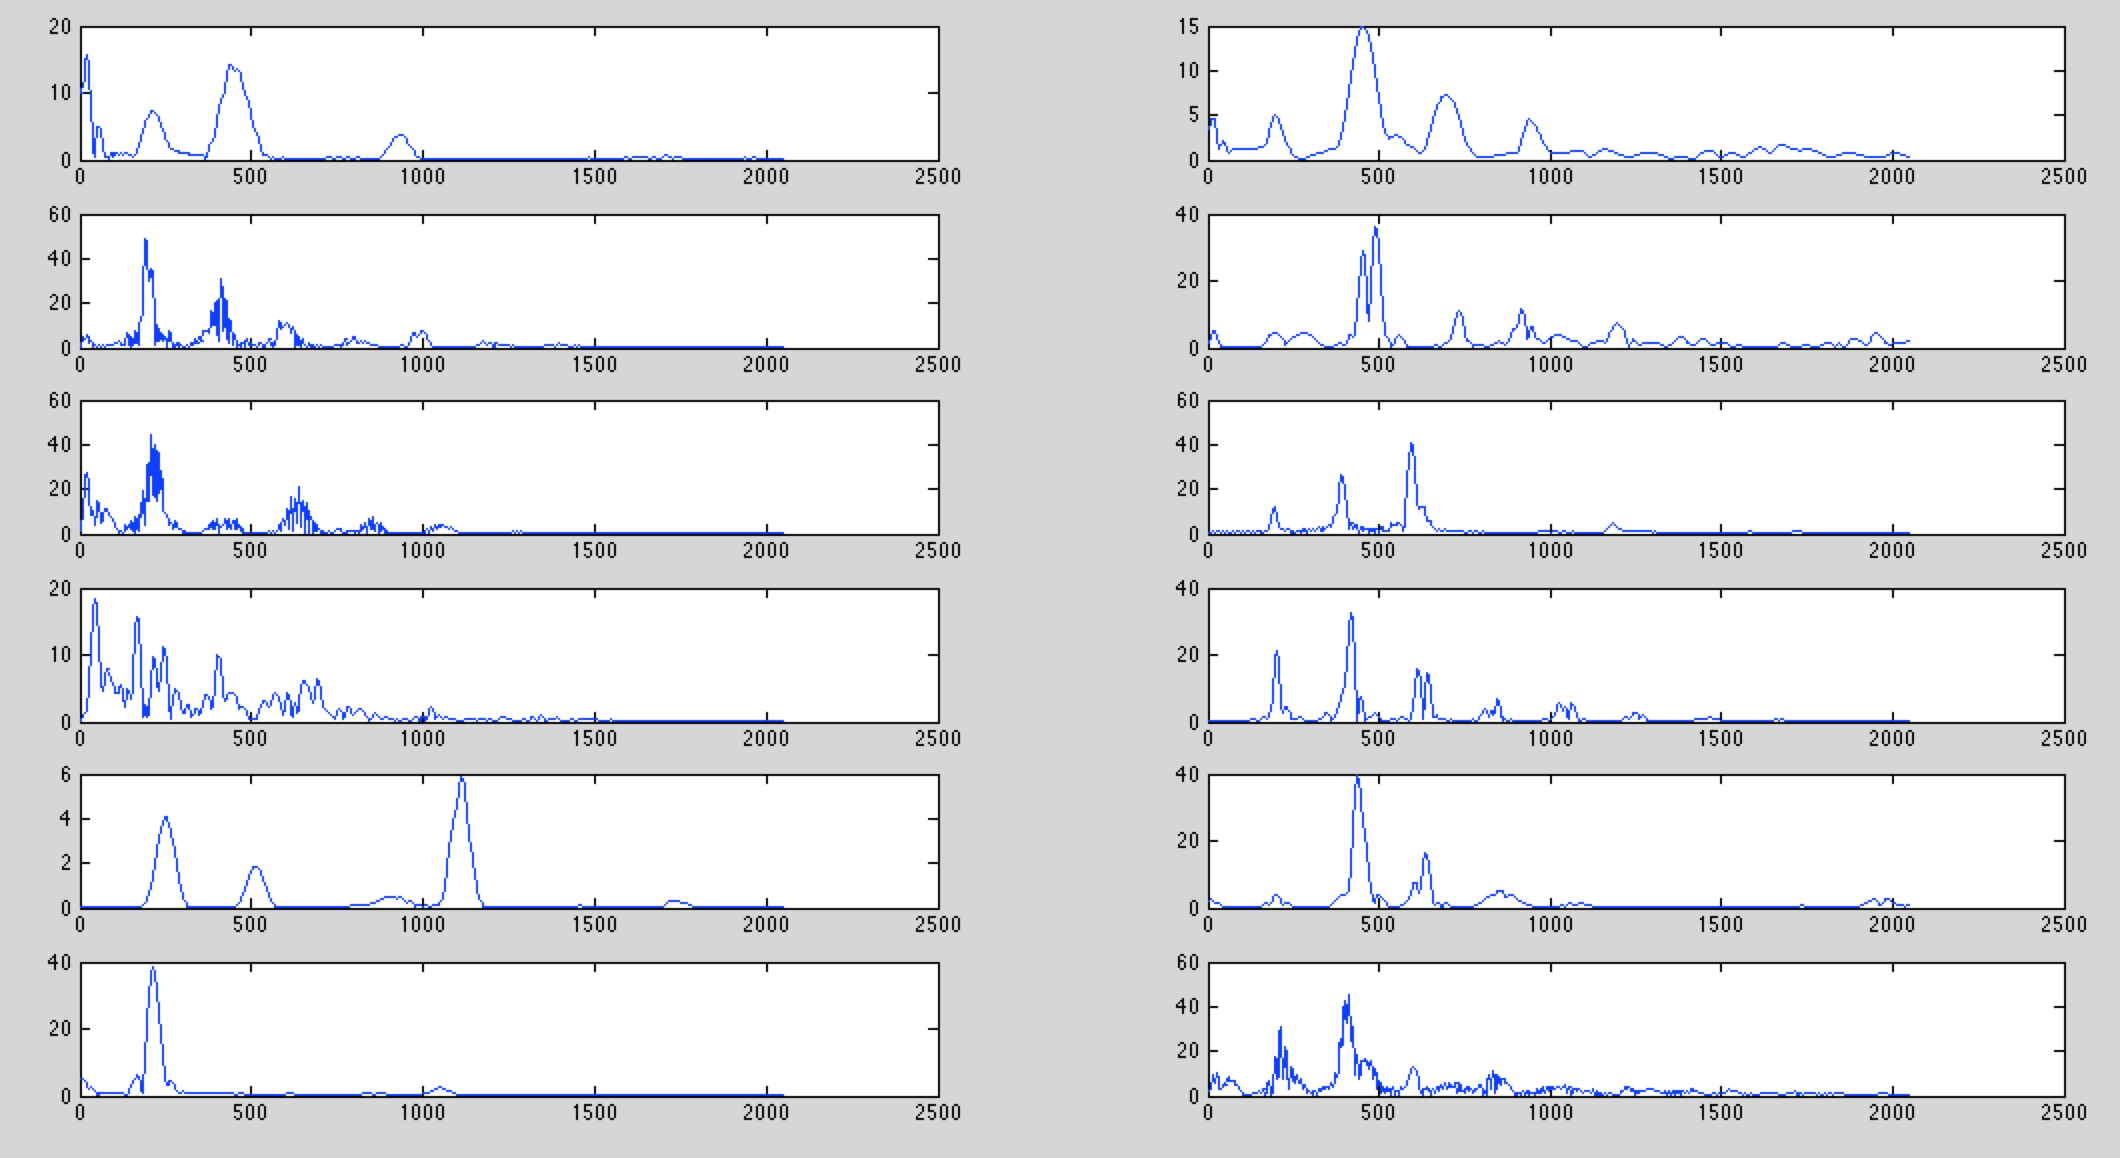
\includegraphics[scale=.4]{PIC/extracted_ffted_class2.png}
\caption{class 2 after fast fourier transform}
\end{figure}

we get the error rate of  0.40182 using Euclidean Distance function and the error rate was 0.39455 using Cosine similarity. The result slightly improve because the feature we extract from the above algorithm is an approximation of the original time series which can also be interpreted as noise reduced version of the original wave. 

\item Using average peak distance as a feature for classification\\
Through observing the above figures, we found out that the distance between two neighbour peaks within one class are similar to each other. Eg. The highest peak in the first graph of Fig3 has coordinate(80, 28), the second nearest peak has coordinate(700, 18), X-coordinate represents the frequency, distance of the two peak's X-coordinate is 620, the distances between two significant peaks are roughly the same within the same class. If we observe class2, The distance is about 202, which is significantly different from the distance in class1. We suppose that we can use the difference of two frequency peaks as the feature of each timeserie, thus to do classification on these timeseries.\\


The algorithm we designed is as follow:\\
\begin{enumerate}
\item Separate the timeseries into 80\% of training data and 20\% test data. \\ 
\item Find two significant and relatively ajacent peaks of each timeserie within the same training class and record each distance as e\_dist.\\
\item Calculate average distance between two peaks found above group by class, record them as avg(dist).\\
\item  Calculate standard diviation between two peaks found above group by class, record them as std(dist).\\
\item  Iterate from step 2, if abs((e\_dist-avg(dist))) > std(dist), delete e\_dist from the class group, proceed to step 3, recalculate the average distance and standard diviation of each class.\\
\item  After iterating several times (we found that 2 times is enough), we finished getting rid of outliers that may influence our result, then we find two significant and relatively ajacent peaks of each timeserie within the same testing class and record each distance as t\_dist.\\
\item  Calculate distance between t\_dist with avg(dist) of each class, classify the testing timeserie to the nearest neighbour (the class that has the shortest distance between t\_dist and avg(dist)).\\
\end{enumerate}
Result: accuracy = 41.36\% (error rate = 0.5864)\\

Means of distances in Training Set is shown in Table 2:\\
\begin{table}[H]
\caption{Mean Distances}
\centering 
\begin{tabular}{c c}
\hline\hline 
Class Label & Mean Distance\\[0.5ex] 
\hline
%heading
    1 & 613.1786 \\
    2 & 198.5263 \\
    3 & 354.4655 \\
    4 & 306.5439 \\
    5 & 509.0625 \\
    6 & 345.2319 \\
    7 & 499.6552 \\
    8 & 374.5667 \\
    9 & 521.0877 \\
   10 & 219.4545 \\
   11 & 166.9000 \\ [1ex]
 
\hline
\end{tabular}
\end{table}

Observing the mean distance of each class above, the reason that the accuracy is low may due to the unobvious differences between the distances, Eg. class 5, class 7 and class 9 have similar distance values, thus it may result in misclassify when classifying testset.\\
Plot class 5, class 7, class 9 on Fig 7,8,9 as below:\\

\begin{figure}[H]
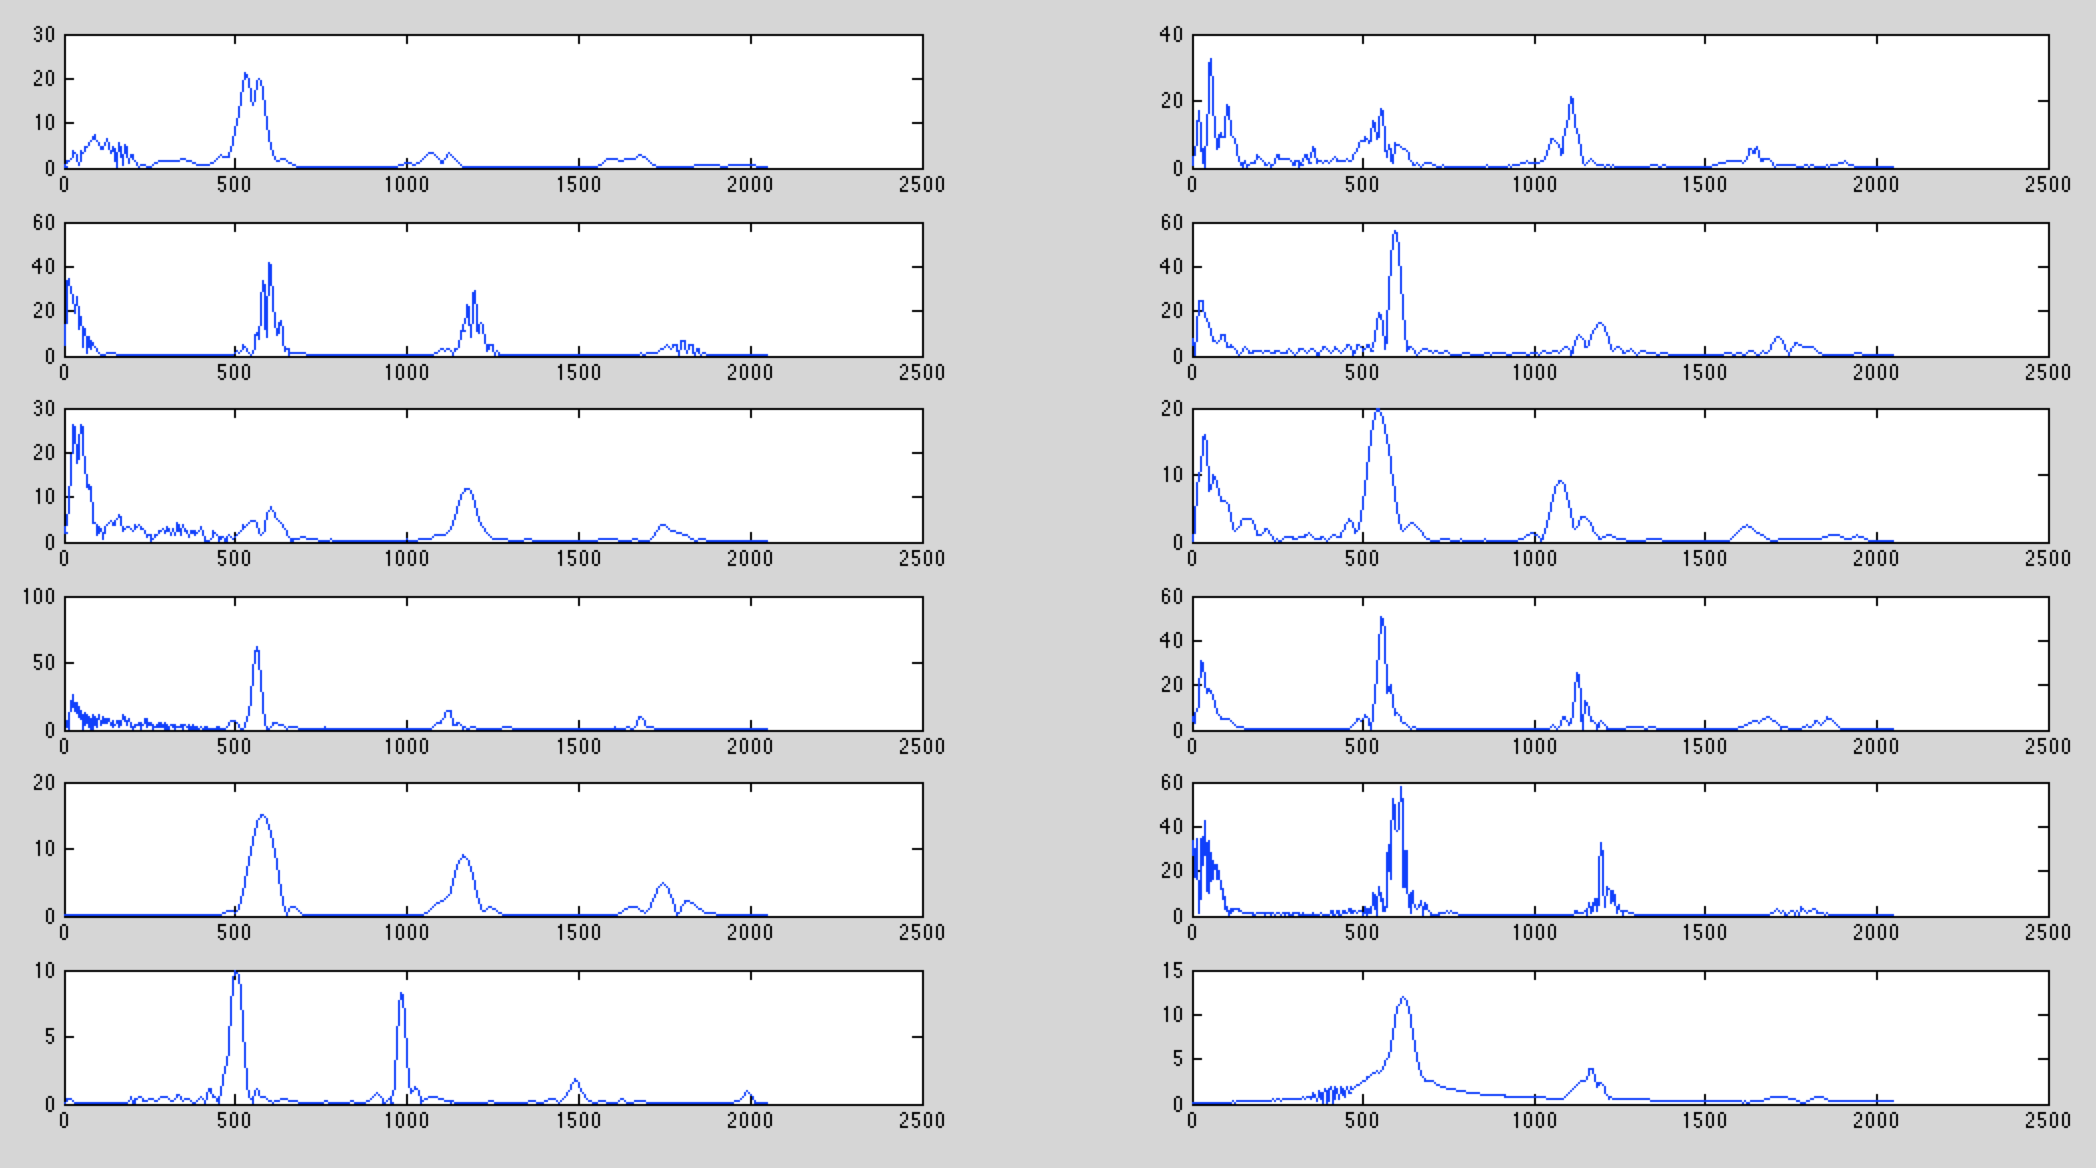
\includegraphics[scale=.4]{PIC/ffted_class5.png}
\caption{class 5 after fast fourier transform}
\end{figure}
\begin{figure}[H]
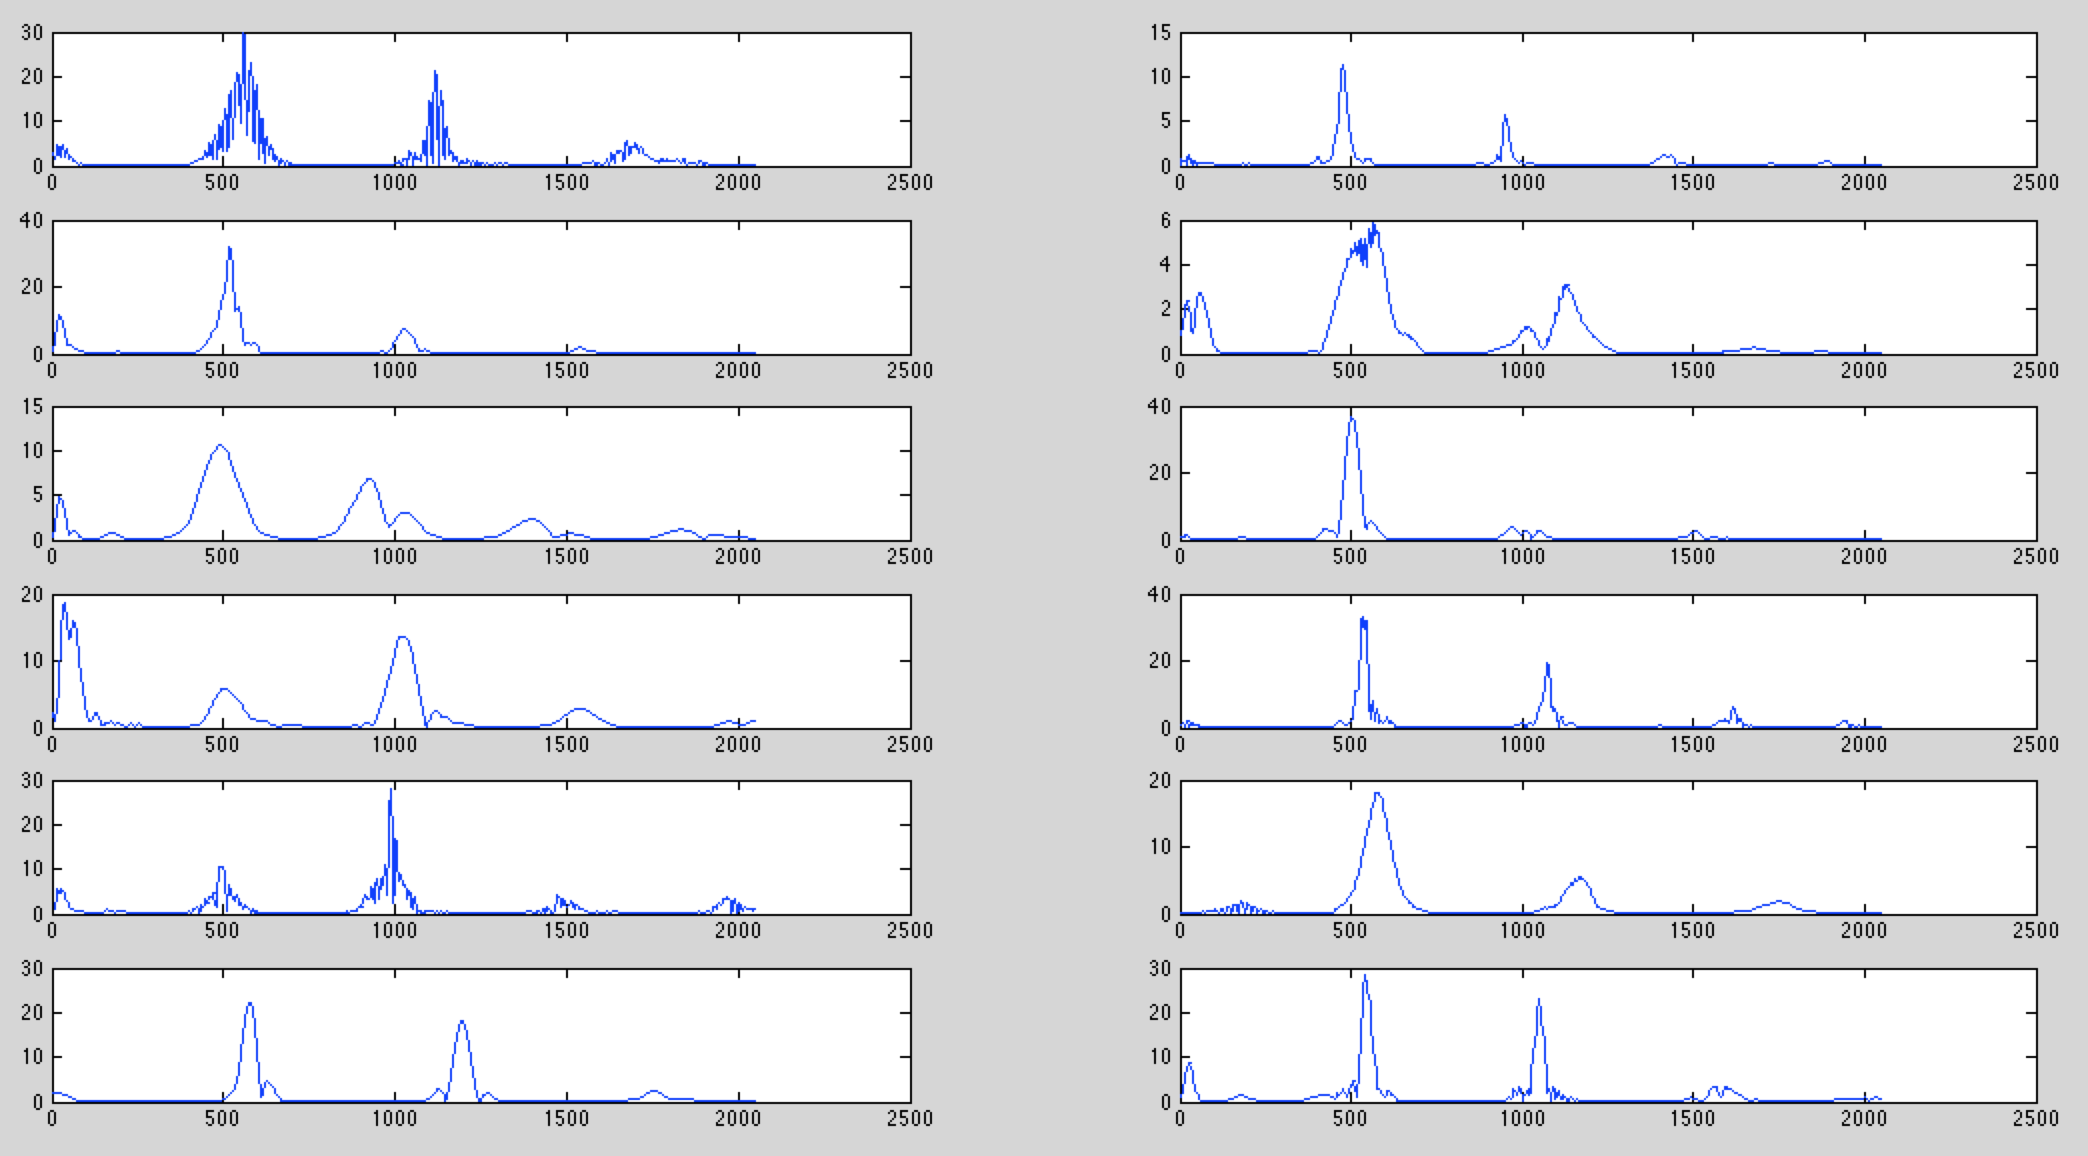
\includegraphics[scale=.4]{PIC/ffted_class7.png}
\caption{class 7 after fast fourier transform}
\end{figure}
\begin{figure}[H]
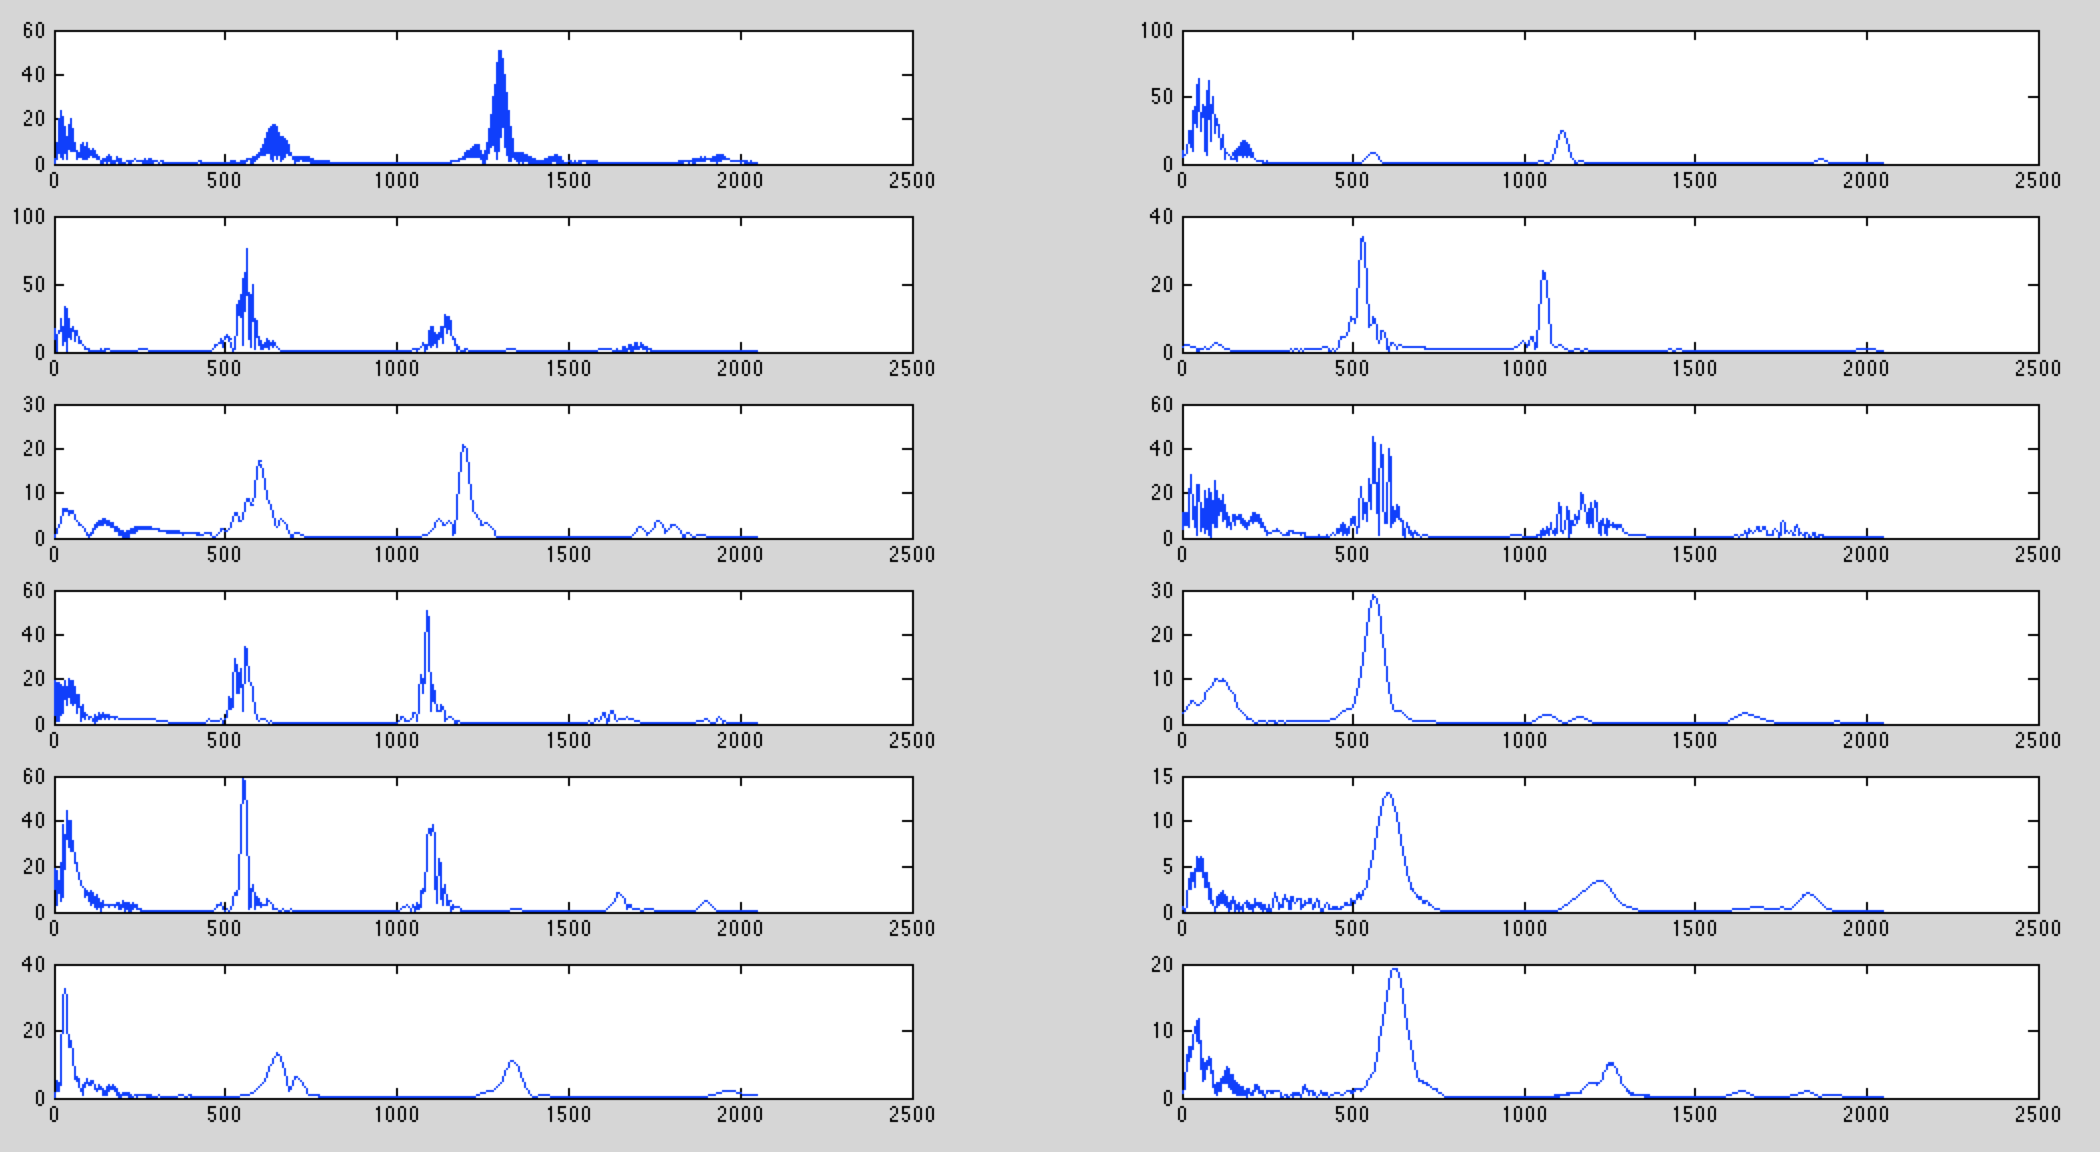
\includegraphics[scale=.4]{PIC/ffted_class9.png}
\caption{class 9 after fast fourier transform}
\end{figure}
From the plots above, we can see that class 5,7,9 have similar distances between the two most significant peaks.\\

\item Use features extracted from frequency domain for classification\\
In the previous method we've found that average distance between peak is not informative enough to classify this dataset. Thus instead of just using average distance between peak, we did experiment on various features extracted from data as follows:\\
Note: we now use LOOCV to do all the remaining experiments and we use standardized Euclidean distance because each feature is in different scale so we have to normalize it first.
\begin{enumerate}
\item Use highest frequency and second highest frequency as two features (this correspond to position in X axis that have highest and second highest peak in Fourier plot). The intuition is that similar insect sound should have nearly the same major frequency. We do not use 3 peaks because many time series have no more than 2 peaks that pass minimum peak height threshold. The error rate is 0.51091 which is better than using average peak distance\\ 
\item Add three more features: distance between highest and second highest peak, amplitude of highest peak and amplitude of second highest peak. We hypothesized that insect sound in the same class should share these charactoristic too. The result error rate for using all five features is 0.48364, sligly better than using two features\\
\item Add number of peak found as another feature. We found that give more weight to this feature ie use square of number of peak give slightly better result. Number of peak found for each wave usually range in 2 to 4. We squares it to make distane further apart. The error rate is 0.46455\\
\item We now have six features for distance function and we want to find out whether we can get rid of some features so we did experiment by removing one of features. We've found that no combination of five features beat performance of six features\\
\item We experimented using one feature at time and get this result
\begin{table}[H]
\caption{Error rate for using single feature }
\begin{center}
    \begin{tabular}{| l | l |}
    \hline
    Feature & Error Rate \\ \hline
    Position of the highest peak & 0.61 \\ \hline
    Position of the second highest peak & 0.71 \\ \hline
    Distance between two peaks & 0.6 \\ \hline
    Amplitude of the highest peak & 0.89 \\ \hline
    Amplitude of the second highest peak & 0.91 \\ \hline
    Number of peaks & 0.91 \\ \hline
    \end{tabular}
\end{center}
\end{table}

Thus we conclude that each feature does not have much discriminative power by itself but we can combine several features to get more information on the data and improve classification accuracy.

\end{enumerate}

\item Custom distance functions by combining different schemes\\
From all of the above experiments. The best result is come from cosine similarity on Fourier transform. We want to improve this by combine this with distance function get from the previous experiment. The methods we tried are as follows: 

\begin{enumerate}
\item 
We combine distance of standardized Euclidean on Fourier Transform wave and tandardized Euclidean on six features extracted from the wave. The error rate was 0.40
\item
We use approximation at level 1 using wavelet transformation to reduce the noise before calculating distance function(FFT, extract features, calculate distance). This came from and observation that if we follow the algorithms proposed by Hui Zhang et al, the approximation at level 1 is enough for this data set. The result of using different mother wavelet are as follows:
\begin{table}[H]
\caption{Error rate from using distance function after wavelet transformation}
\centering 
\begin{tabular}{c c}
\hline\hline 
Wavelet used & Error Rate\\[0.5ex] 
\hline
%heading
    haar & 0.40273 \\
    db4 & 0.38909 \\
    db8 & 0.40273 \\
    db12 & 0.38727 \\
    db16 & 0.39364 \\
    coif1 & 0.40273 \\
    coif3 & 0.39273 \\
    coif5 & 0.39091 \\ [1ex]
 
\hline
\end{tabular}
\end{table}
\end{enumerate}

\item Adding standardized euclidean distance function on time series in time domain (with shifting to match position of the sound).\\ We add this as a bias in case that some time series are very differrent in time domain but happen to be similar in frequency domain. In first attempt we just add three custom distance function together with the same weight ie distance using features + distance in frequency domain + distance in time domain. The error rate was 0.44727. The result get worse because distance in time domain does not perform as well as the other two distance functions, so we put more weight to distance in frequency domain and features using this formula: cube(distance using features) + cube(distance in frequency domain) + distance in time domain. \\The error rate was 0.38455 which is the best we get from all experiments.
\begin{flushleft}
\textbf{Visualization}\\
\end{flushleft}

\begin{enumerate}
\item SVD\\
We use SVD to reduce the dimensional of transformed signal to two dimension by keeping only two strongest concepts. We assign different colors to each insect classes and plot the result using scatter plot.
\begin{center}
Experiment result:\\
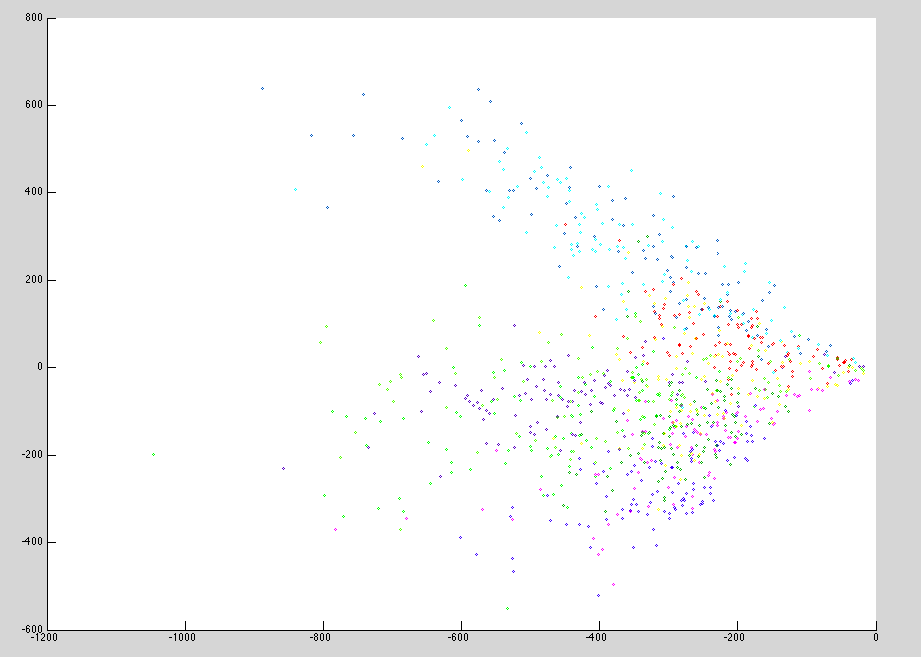
\includegraphics[scale=.4]{PIC/fftsvdplot.png}
\caption{Visualization using SVD}
\end{center}
\begin{flushleft}We can detect some patterns from the plot. For example,the red class clustered at the central right part of the graph, the density of the red class looks higher than any other classes. The dark blue class scattered within the right part of the graph, the light blue class seems linearly distributed. The high density cluster in the right center part area is a mixture of many classes so it's hard to classify.
\end{flushleft}


\item MDS\\
Using MDS with custom distance function in frequency domain we got below result:

\begin{figure}[H]
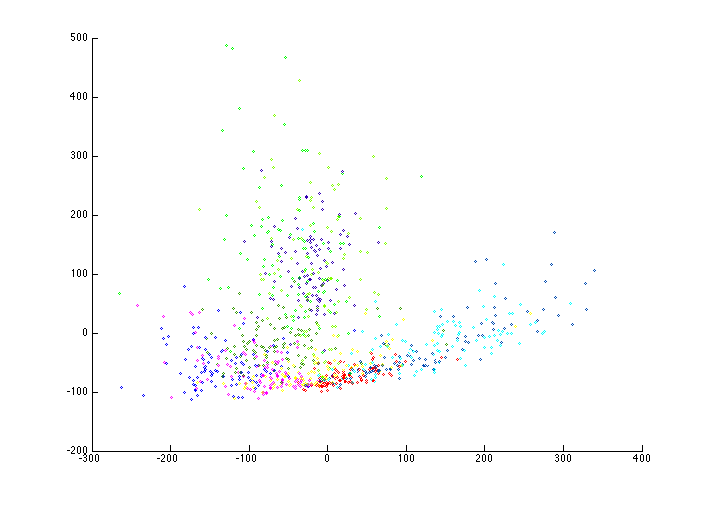
\includegraphics[scale=.6]{PIC/mds_fft_plot.png}
\caption{Visualization Using MDS}
\end{figure}

We can detect several clusters from this plot. The light blue cluster is concentrate on the right side and look linear. Light green is on the upper side. On the left we spot pink cluster and a group of dark blue. Red and yellow concentrate on the bottom part.

\item FastMap\\
Using Fastmap with custom distance function in frequency domain we got below result:

\begin{figure}[H]
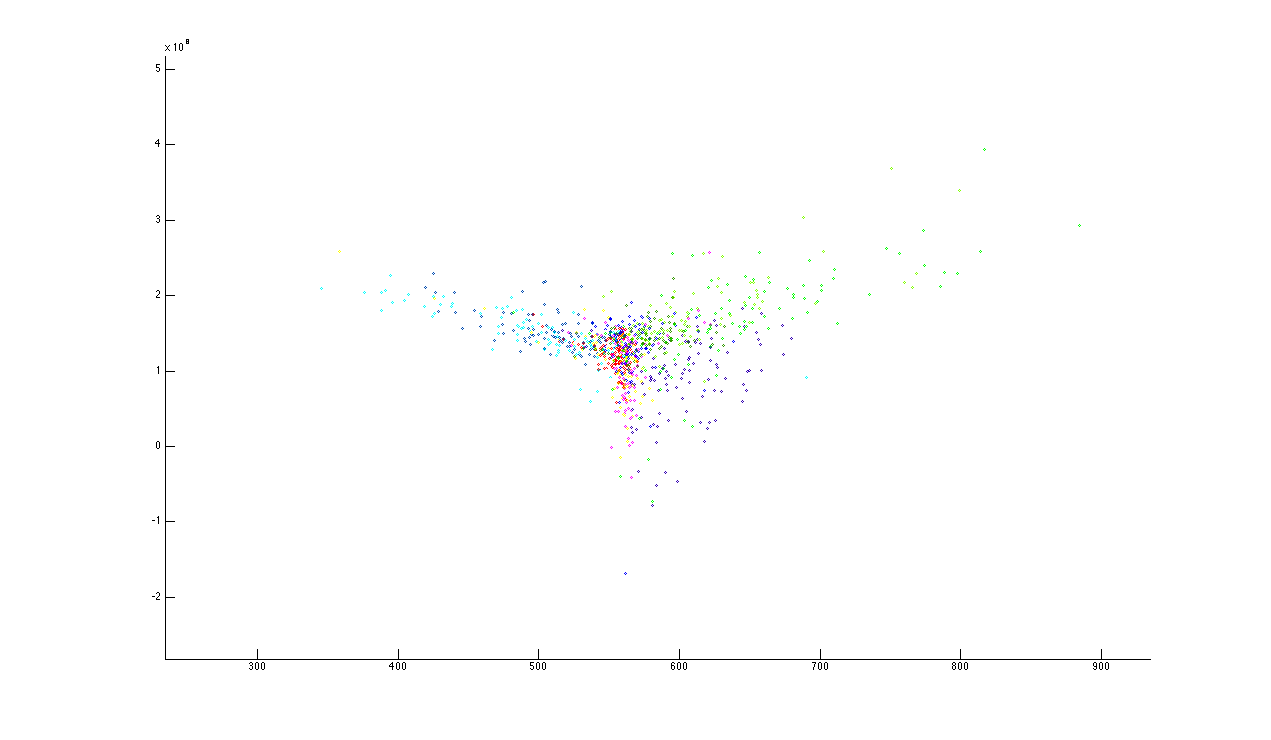
\includegraphics[scale=.4]{PIC/fastmap_fft_plot.png}
\caption{Visualization Using FastMap}
\end{figure}

We can spot more or less similar pattern in FastMap and MDS. Green cluster is now on the right side; while light blue is on the left. Pink cluster is on the down side near the center and most of the cluster concentrate on the center. The drak blue seem to be scatter around. The dense area in the center is hard for classification.
\end{enumerate}
\textbf{Anomaly Detection}\\
We used LOF as the algorithm of detecting anomalies. The algorithm indicates that the detection of anomalies can depend on how isolated the object is with respect to the
surrounding neighborhood. Through calculating each object's Euclidean distance with other objects and set the number of k(k-neighbours) from 10 to 100, after comparing the distances, we found four wav files' LOF value always ranked top four, so we believe these four are anomalies:\\
00066.wav\\
00017.wav\\
00128.wav\\
00007.wav\\
Their LOF value to other objects are significantly larger. The distances are:\\
18.7306\\
16.3915\\
14.1451\\
2.6638\\
while others all have the LOF value less than 2.
The outliers found above are plotted as follows:\\
\begin{figure}[H]
\centering
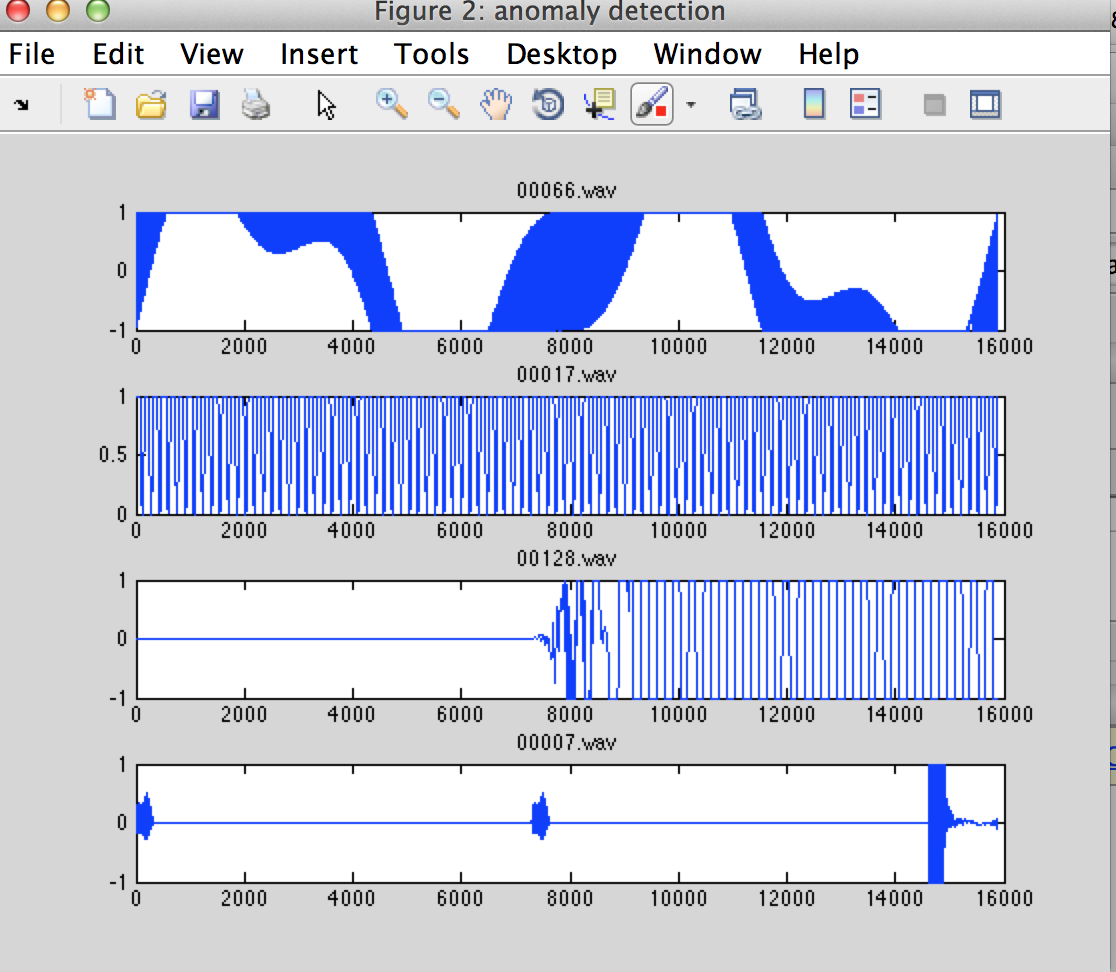
\includegraphics[scale=.6]{PIC/outliers}
\caption{Outliers}
\end{figure}
Compare with the normal ones shown below:\\
\begin{figure}[H]
\centering
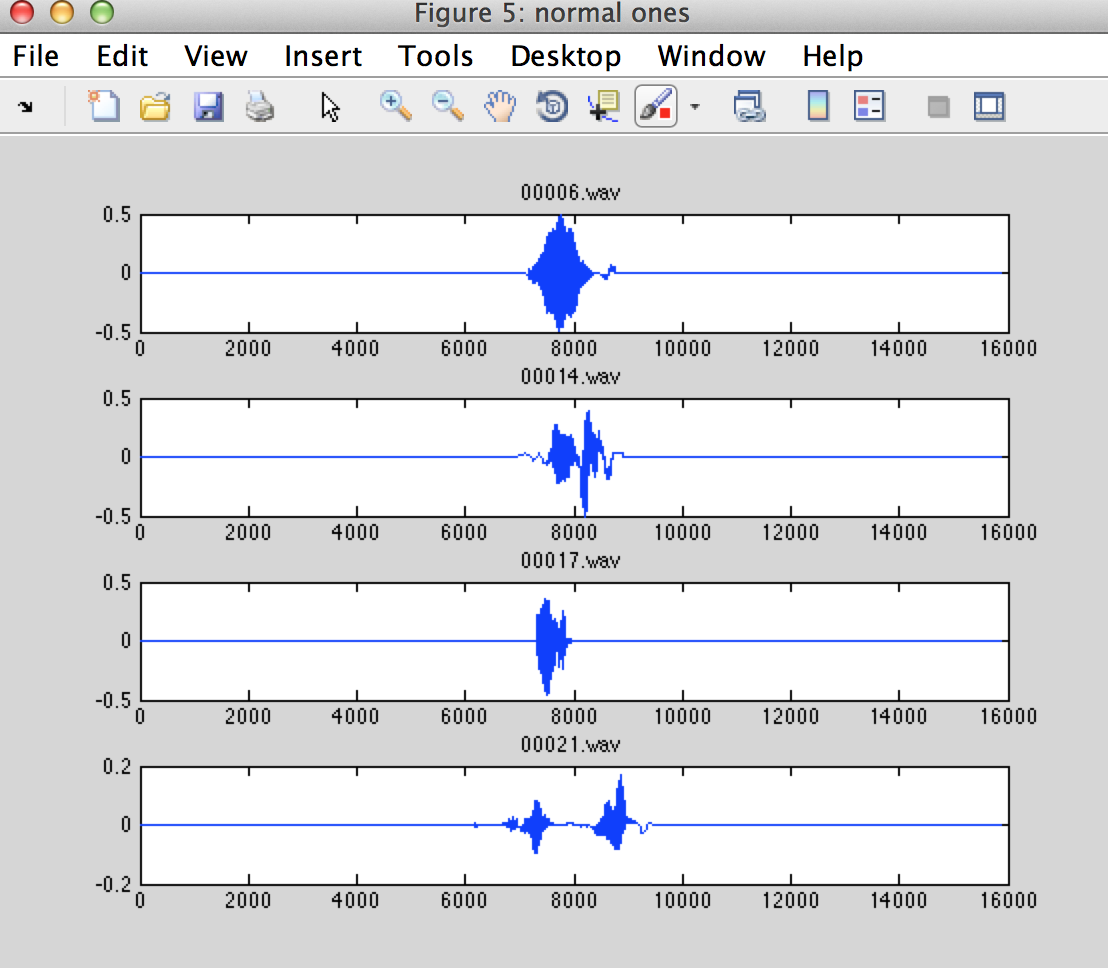
\includegraphics[scale=.6]{PIC/normal}
\caption{Normal ones}
\end{figure}
We believe that we correctly selected the anomalies.